\documentclass{beamer}
\usetheme{metropolis}           % Use metropolis theme
\usepackage[utf8]{inputenc}
\usepackage[spanish]{babel}
\usepackage{subcaption}
%%package para bibliografía
\usepackage{natbib}
\usepackage[american,siunitx]{circuitikz}
\usepackage[version=4]{mhchem}
\usepackage{caption}
\captionsetup{font=scriptsize,labelfont=scriptsize}
\captionsetup[subfigure]{font=scriptsize,labelfont=scriptsize}
\usepackage{pgfplots}
\usepackage{pgfplotstable,tabularx,booktabs}
\usepgfplotslibrary{units}
\usepackage{multirow}
\usepackage{xcolor,colortbl}
\definecolor{LightCyan}{rgb}{0.88,1,1}

\let\clipbox\relax
\usepackage{adjustbox}

\newcommand{\plotwidth}{0.2\textwidth}
\newcommand{\plotscale}{0.4}

\captionsetup{subrefformat=parens}

\setbeamercovered{invisible}
\setbeamercovered{%
	again covered={\opaqueness<1->{10}}}
\usepackage[skins]{tcolorbox}
\graphicspath{{Imagenes/}}

\tikzset{
	invisible/.style={opacity=0},
	visible on/.style={alt={#1{}{invisible}}},
	alt/.code args={<#1>#2#3}{%
		\alt<#1>{\pgfkeysalso{#2}}{\pgfkeysalso{#3}} % \pgfkeysalso doesn't change the path
	},
}

%nombre de muestras:
\newcommand{\mSustratoAcero}{SusAc }
\newcommand{\mPolvoAcero}{PolvoAc }
\newcommand{\mPolvoAceroPMMA}{PolvoAc+pmma }
\newcommand{\mPapelAcero}{PapelAc }
\newcommand{\mLiofilizadoAcero}{LioAc }
\newcommand{\mSustratoNiquel}{SusNi }
\newcommand{\mPolvoNiquel}{PolvoNi }
\newcommand{\mPolvoNiquelPMMA}{PolvoNi+pmma }

\definecolor{RYB1}{RGB}{228,26,28}
\definecolor{RYB2}{RGB}{55,126,184}
\definecolor{RYB3}{RGB}{77,175,74}
\definecolor{RYB4}{RGB}{152,78,163}
\definecolor{RYB5}{RGB}{255,127,0}
\definecolor{RYB6}{RGB}{255,255,51}
\definecolor{RYB7}{RGB}{166,86,40}
\definecolor{ce4edc3}{RGB}{228,237,195}
\definecolor{cfe9999}{RGB}{254,153,153}
\definecolor{c575757}{RGB}{87,87,87}
\definecolor{c43d8ff}{RGB}{67,216,255}
\definecolor{c323232}{RGB}{50,50,50}
\definecolor{c71d89a}{RGB}{113,216,154}
\definecolor{cbfbfbf}{RGB}{191,191,191}
\definecolor{c252525}{RGB}{37,37,37}

\pgfplotscreateplotcyclelist{colorbrewer-RYB}{
	{RYB1},every mark/.append style={fill=RYB1!80!black},mark=*\\
	{RYB2},every mark/.append style={fill=RYB2!80!black},mark=square*\\
	{RYB3},every mark/.append style={fill=RYB3!80!black},mark=diamond*\\
	{RYB4},every mark/.append style={fill=RYB4!80!black},mark=triangle*\\
	{RYB5},every mark/.append style={fill=RYB5!80!black},mark=pentagon*\\
	{RYB6},every mark/.append style={fill=RYB6!80!black},mark=o\\
	{RYB7},every mark/.append style={fill=RYB7!80!black},mark=square\\
}


\pgfplotsset{
	compat=1.15,
	CVStyle/.style={
		title=Voltametría Cíclica,
		domain=-0.8:0.8,
		xtick distance=0.4,
		minor tick num=1,
		ylabel={Densidad de corriente [A/g]},
		xlabel={Voltaje [V]},
		every axis legend/.append style={
			font=\normalsize,
			at={(0.98,0.02)},
			anchor=south east,
		},
		legend entries={25mV/s,50mV/s,100mV/s,200mV/s,400mV/s},
		cycle list name=colorbrewer-RYB,
		no markers,
	},
	SCStyle/.style={
		title=Capacidad Específica,
		domain=25:400,
		ylabel={Capacidad específica [F/g]},
		xlabel={Velocidad de barrido [mV/s]},
		every axis legend/.append style={
			font=\tiny,
			at={(0.98,0.98)},
			anchor=north east,
		},
		legend entries={Antes, Después},
		cycle list name=colorbrewer-RYB,
		every mark/.append style={
			fill opacity=0.5,
			draw opacity=0.5,}
	},
	EISStyle/.style={
		title=Espectro de impedancia electroquímica,
		domain=0:50,
		ylabel={-Z imag [$\Omega$]},
		xlabel={Z real [Ohm]},
		cycle list name=colorbrewer-RYB,	
	},
	CCDStyle/.style={
		title=Carga y descarga cíclica,
		ylabel={Voltaje [V]},
		xlabel={Tiempo [s]},
		cycle list name=colorbrewer-RYB,
		mark size = 1pt,
		line width = 0.1pt,
		%		only markers,
		every axis legend/.append style={
			font=\tiny,
			at={(0.98,0.02)},
			anchor=south east,
		},
		legend entries={Primeros ciclos, Últimos ciclos},
	},
}

\pgfplotsset{
	/pgfplots/bar  cycle  list/.style={/pgfplots/cycle  list={%
			{RYB1,fill=RYB1!80!black,mark=*},
			{RYB2,fill=RYB2!80!black,mark=square*},
			{RYB3,fill=RYB3!80!black,mark=diamond*},
			{RYB4,fill=RYB4!80!black,mark=triangle*},
			{RYB5,fill=RYB5!80!black,mark=*},
			{RYB6,fill=RYB6!80!black,mark=square*},
			{RYB7,fill=RYB7!80!black,mark=diamond*},
		}
	},
}
\title{Síntesis de grafeno por medios químicos}
\subtitle{y supercondensadores basados en grafeno}
\date{\today}
\institute{Universidad de Santiago de Chile\\ Laboratorio de Nanosíntesis}
\begin{document}
	\author[Carlos Eugenio]{\begin{tabular}{r@{ }l} 
			Autor:      & Carlos Eugenio \\[1ex] 
			Profesor guía: & Dinesh Pratap Singh
	\end{tabular}}
	\maketitle
	\begin{frame}
		\frametitle{Table of Contents}
		\tableofcontents[currentsection]
	\end{frame}

	\section{Objetivos}
	\subsection{Objetivo general}
	\begin{frame}{Objetivos}
	Objetivo general
		\begin{itemize}
			\item Sintetizar óxido de grafeno reducido, para su utilización en electrodos de supercondensadores.
		\end{itemize}
	
	\end{frame}

	\subsection{Objetivos específicos}
	\begin{frame}{Objetivos}
	Objetivos específicos
		\begin{itemize}[<+>]
			\item Sintetizar óxido de grafeno (GO), a partir de grafito natural mediante un proceso químico; para su posterior reducción y obtención de óxido reducido de grafeno (rGO).
			\item Fabricar electrodos de óxido de grafeno reducido con diferentes métodos, para su posterior caracterización electroquímica.
			\item Diseñar y construir una celda de pruebas de supercondensadores para estudiar el desempeño de diferentes electrodos fabricados.
			\item Elaborar una metodología de medición electroquímica para cuantificar y comparar el desempeño de los diferentes electrodos fabricados. 
		\end{itemize}
	\end{frame}

	\section{Introducción}
	\begin{frame}{Introducción}
		\subsection{Nanociencia}
		\begin{figure}[h!]
			\centering
			\fbox{
				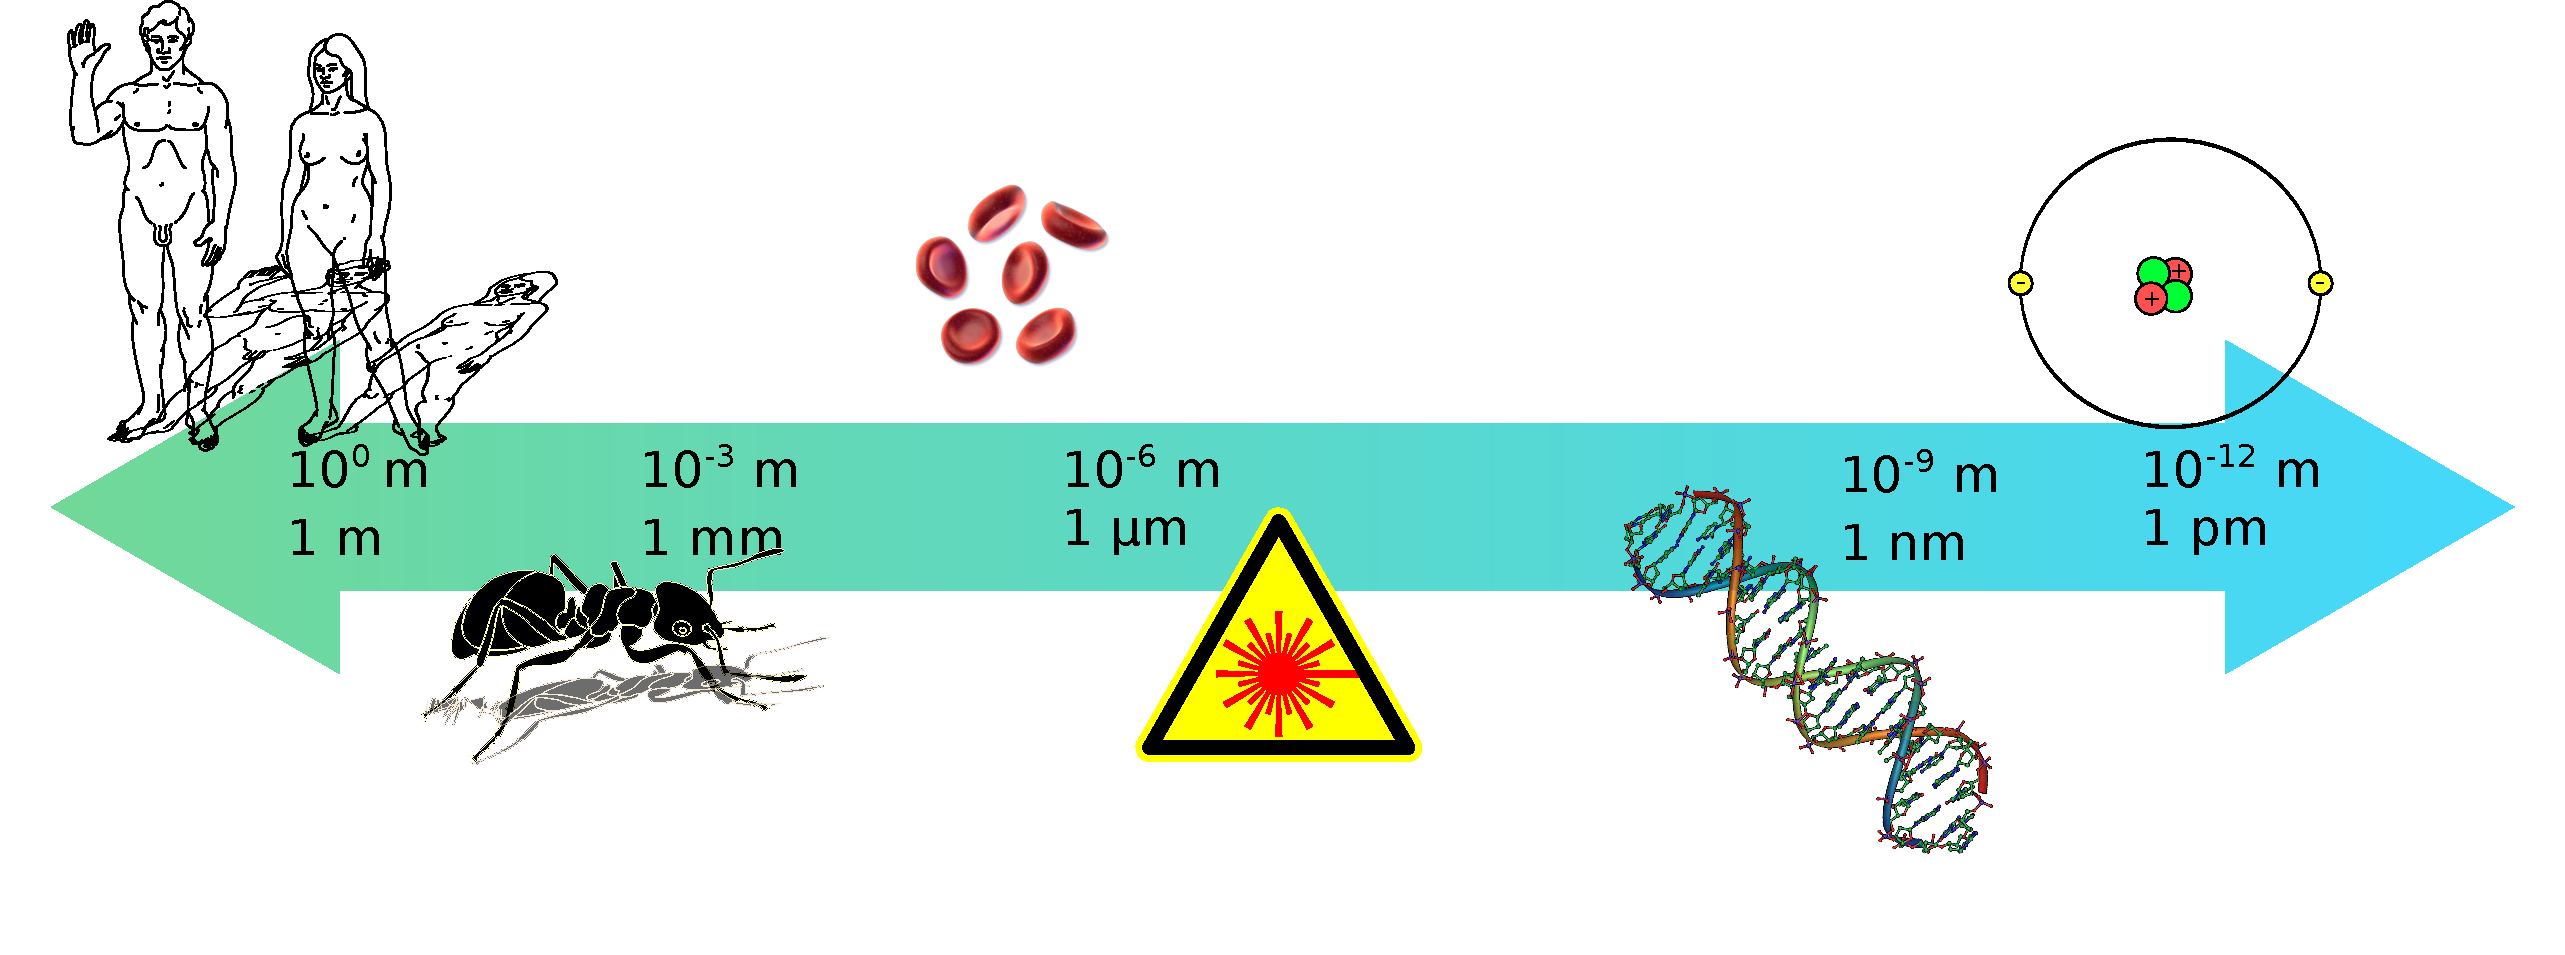
\includegraphics[width=0.9\textwidth]{scale.pdf}
			}
			\caption[Comparativa de ódenes de magnitud desde metros hasta picometros]{Comparativa de órdenes de magnitud. De izquierda a derecha: Escala humana, 1-2 m. Insectos, 10 cm - 1 mm. Glóbulos rojos, 6 $\mathrm{\mu}$m. Longitud de onda de luz visible, 780-380 nm. Transistores en un microprocesador, 100 - 10 nm. Doble hélice de ADN, 2 nm. Radio atómico de un átomo de helio, 31 pm.}
			\label{fig:scale}
		\end{figure}
	\end{frame}

	\begin{frame}{Introducción}
		\begin{figure}
			\centering
			\begin{subfigure}[b]{0.15\textwidth}
				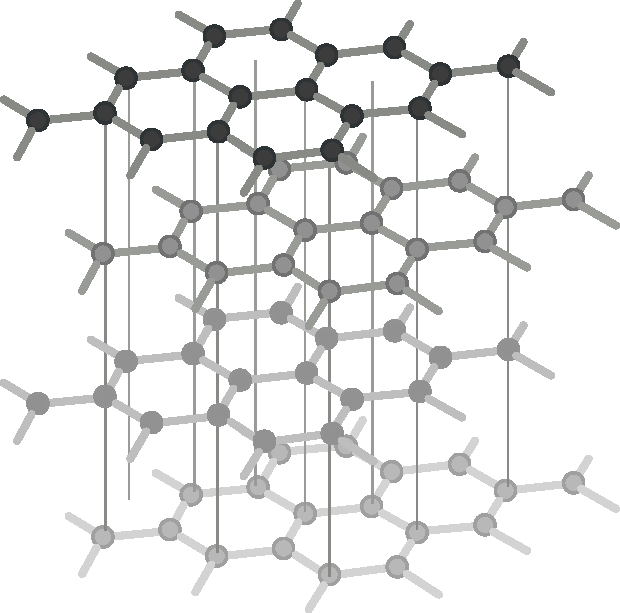
\includegraphics[width=\textwidth]{graphite_structure.pdf}
				\caption{}
				\label{fig:graphite_struct}
			\end{subfigure}
			\begin{subfigure}[b]{0.15\textwidth}
				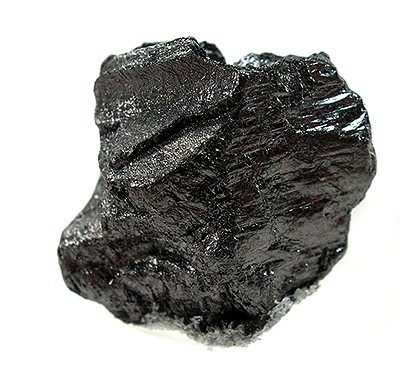
\includegraphics[width=\textwidth]{graphite_image.jpg}
				\caption{}
				\label{fig:graphite_image}
			\end{subfigure}
			\begin{subfigure}[b]{0.15\textwidth}
				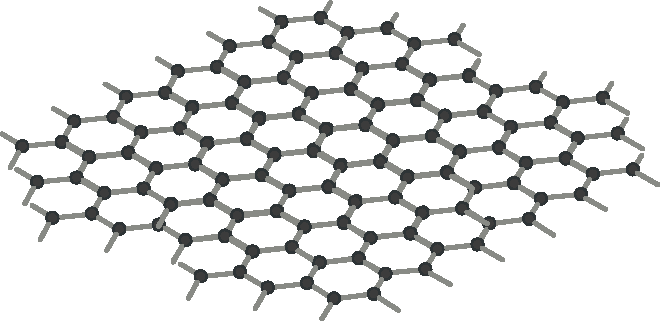
\includegraphics[width=\textwidth]{graphene_structure.pdf}
				\caption{}
				\label{fig:graphene_struct}
			\end{subfigure}
			\begin{subfigure}[b]{0.15\textwidth}
				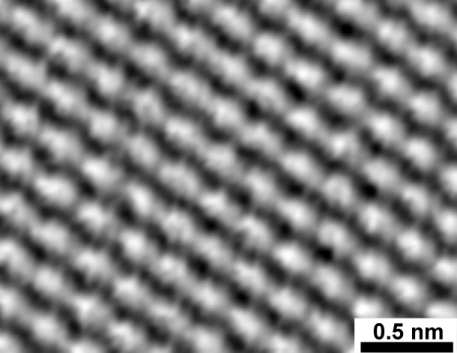
\includegraphics[width=\textwidth]{graphene_image.jpg}
				\caption{}
				\label{fig:graphene_image}
			\end{subfigure}
			\\
			\begin{subfigure}[b]{0.15\textwidth}
				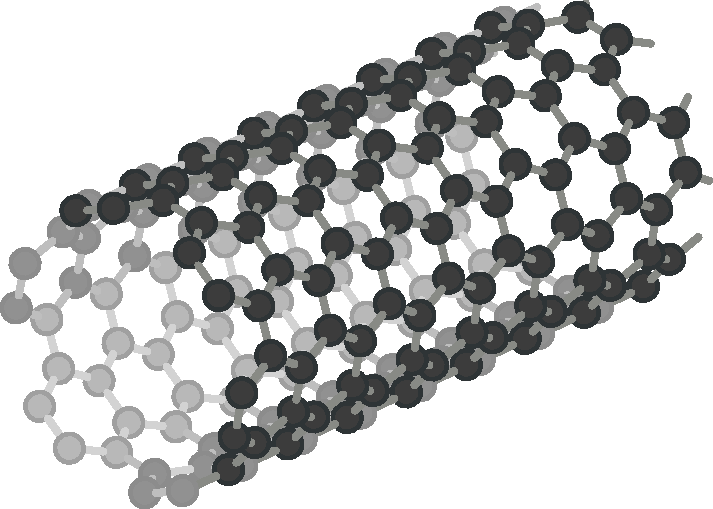
\includegraphics[width=\textwidth]{cnt_structure.pdf}
				\caption{}
				\label{fig:cnt_struct}
			\end{subfigure}
			\begin{subfigure}[b]{0.15\textwidth}
				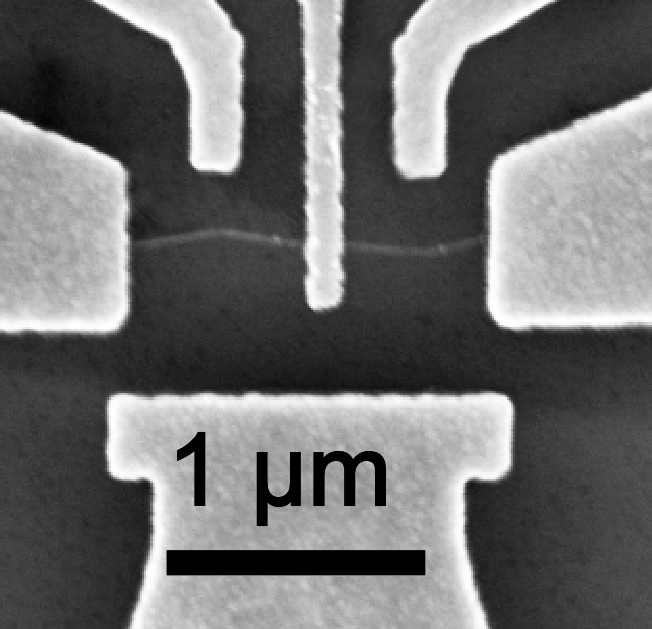
\includegraphics[width=\textwidth]{cnt_image.png}
				\caption{}
				\label{fig:cnt_image}
			\end{subfigure}
			\begin{subfigure}[b]{0.15\textwidth}
				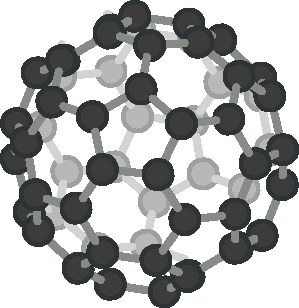
\includegraphics[width=\textwidth]{fullerene_structure.pdf}
				\caption{}
				\label{fig:fullerene_structure}
			\end{subfigure}
			\begin{subfigure}[b]{0.15\textwidth}
				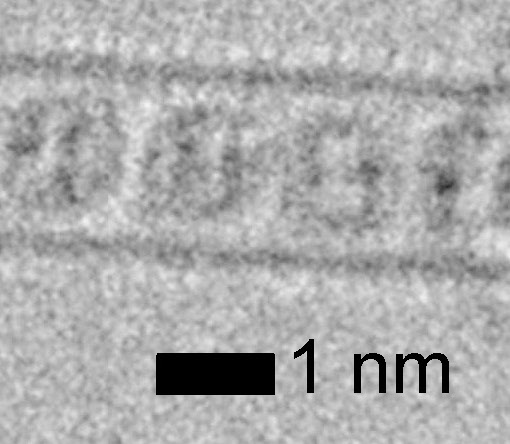
\includegraphics[width=\textwidth]{fullerene_image.jpg}
				\caption{}
				\label{fig:fullerene_image}
			\end{subfigure}
			\caption[Alótropos del carbono mostrando las diferentes dimensionalidades de los nanomateriales]{\subref{fig:graphite_struct} y \subref{fig:graphite_image} grafito natural. \subref{fig:graphene_struct} y \subref{fig:graphene_image} grafeno(Frank Trixler, LMU/CeNS: Organic Semiconductor Group). \subref{fig:cnt_struct} y \subref{fig:cnt_image} nanotubo de carbono, (Pavlos Apostolidis, London Centre for Nanotechnology, Department of Physics \& Astronomy). \subref{fig:fullerene_structure} y \subref{fig:fullerene_image} fullereno\citep{Gimenez2011}.}
			\label{fig:carbon_allotropes}
		\end{figure}
	\end{frame}

	\subsection{Grafeno}
	\begin{frame}{Grafeno}
		\begin{figure}
			\centering
			\fbox{
				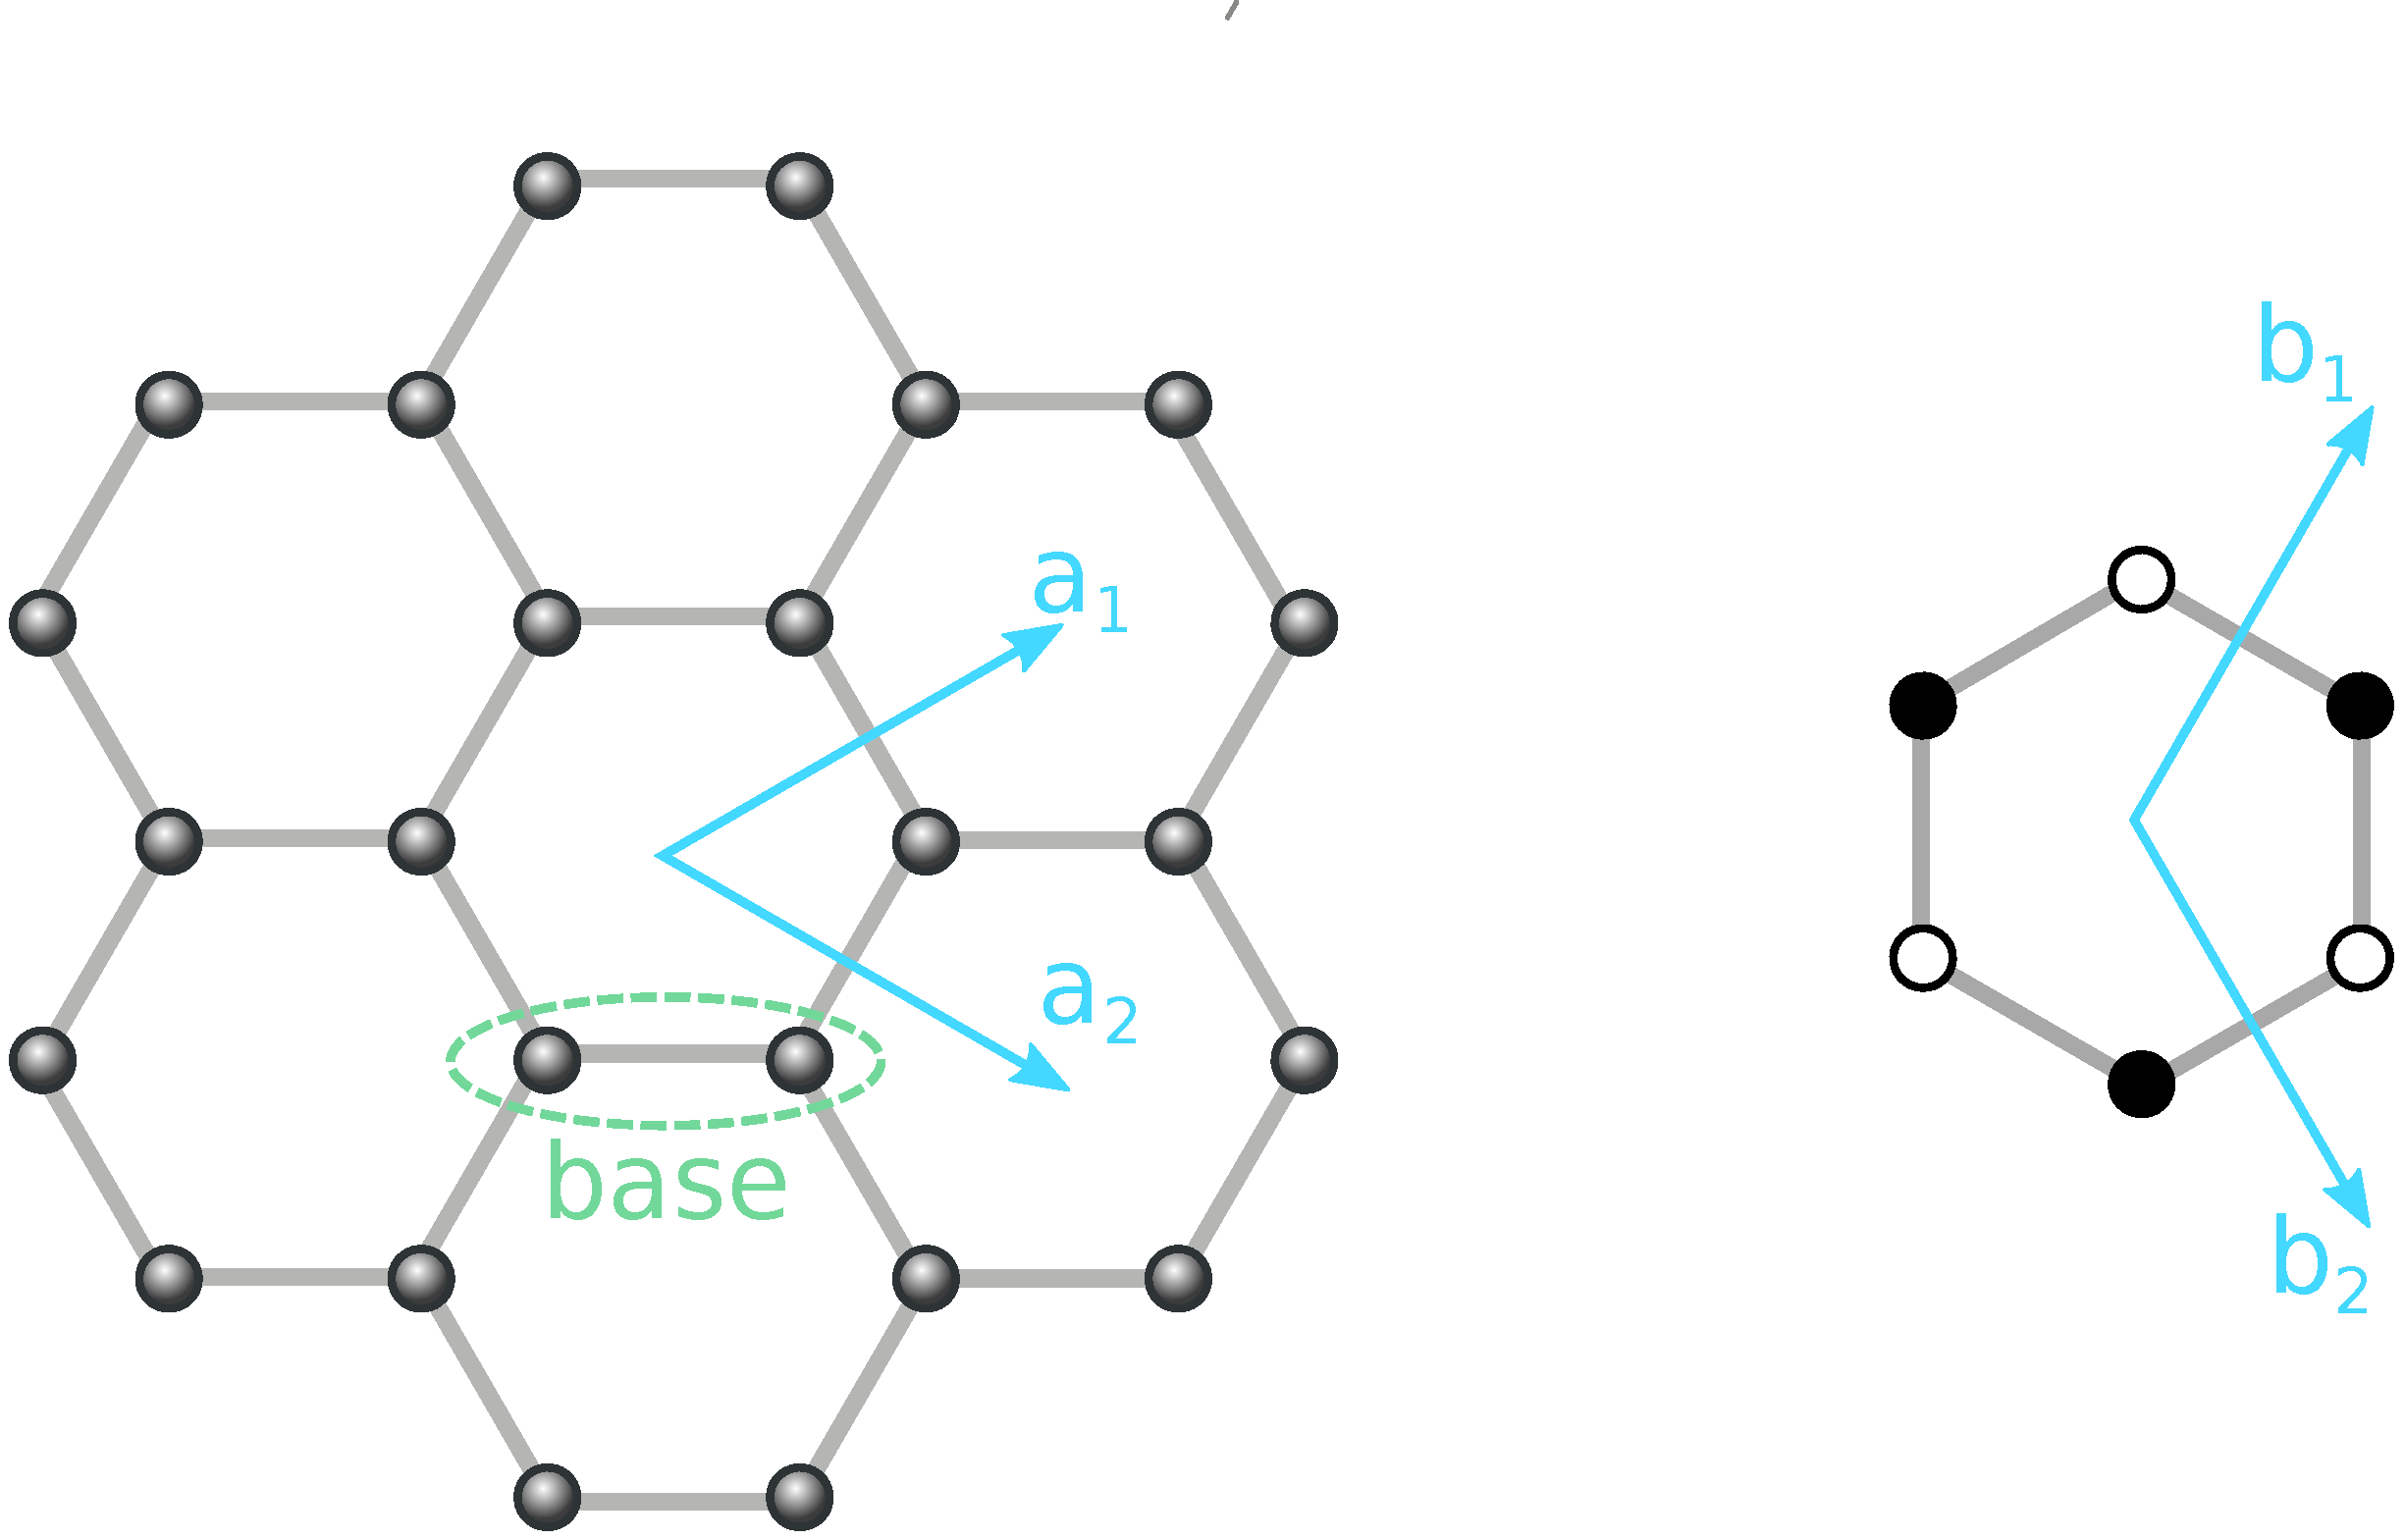
\includegraphics[width=0.75\textwidth]{graphene_lattice.pdf}
			}
			\caption[Estructura cristalina del grafeno]{Izquierda: Red de grafeno en espacio real. Derecha: Red en espacio recíproco.}
			\label{fig_graphene_lattice}
		\end{figure}
	\end{frame}
	
	\subsection{Supercondensadores}
	\begin{frame}{Supercondensadores}
		\begin{figure}
			\centering
			\fbox{
				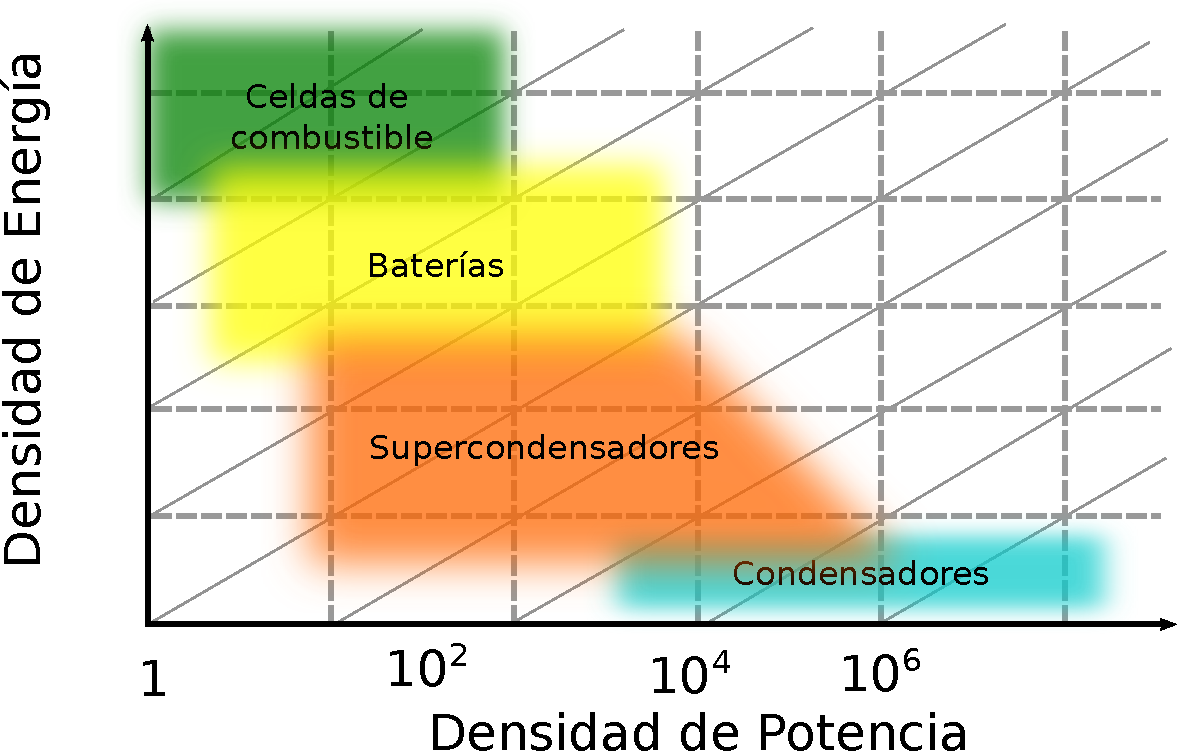
\includegraphics[width = 0.7\textwidth]{ragone.pdf}
			}
			\caption[Diagrama de Ragone, diferentes tecnologías de almacenamiento de energía]{El diagrama de Ragone compara diferentes tecnologías de almacenamiento de energía de acuerdo a su densidad de potencia y densidad de energía.}
			\label{fig:ragone}
		\end{figure}
	\end{frame}
\newcommand{\clipradius}{2cm}
	\section{Ruta de síntesis}
	\begin{frame}{Ruta de síntesis}
%		\begin{figure}
%			\centering
%			\fbox{
%				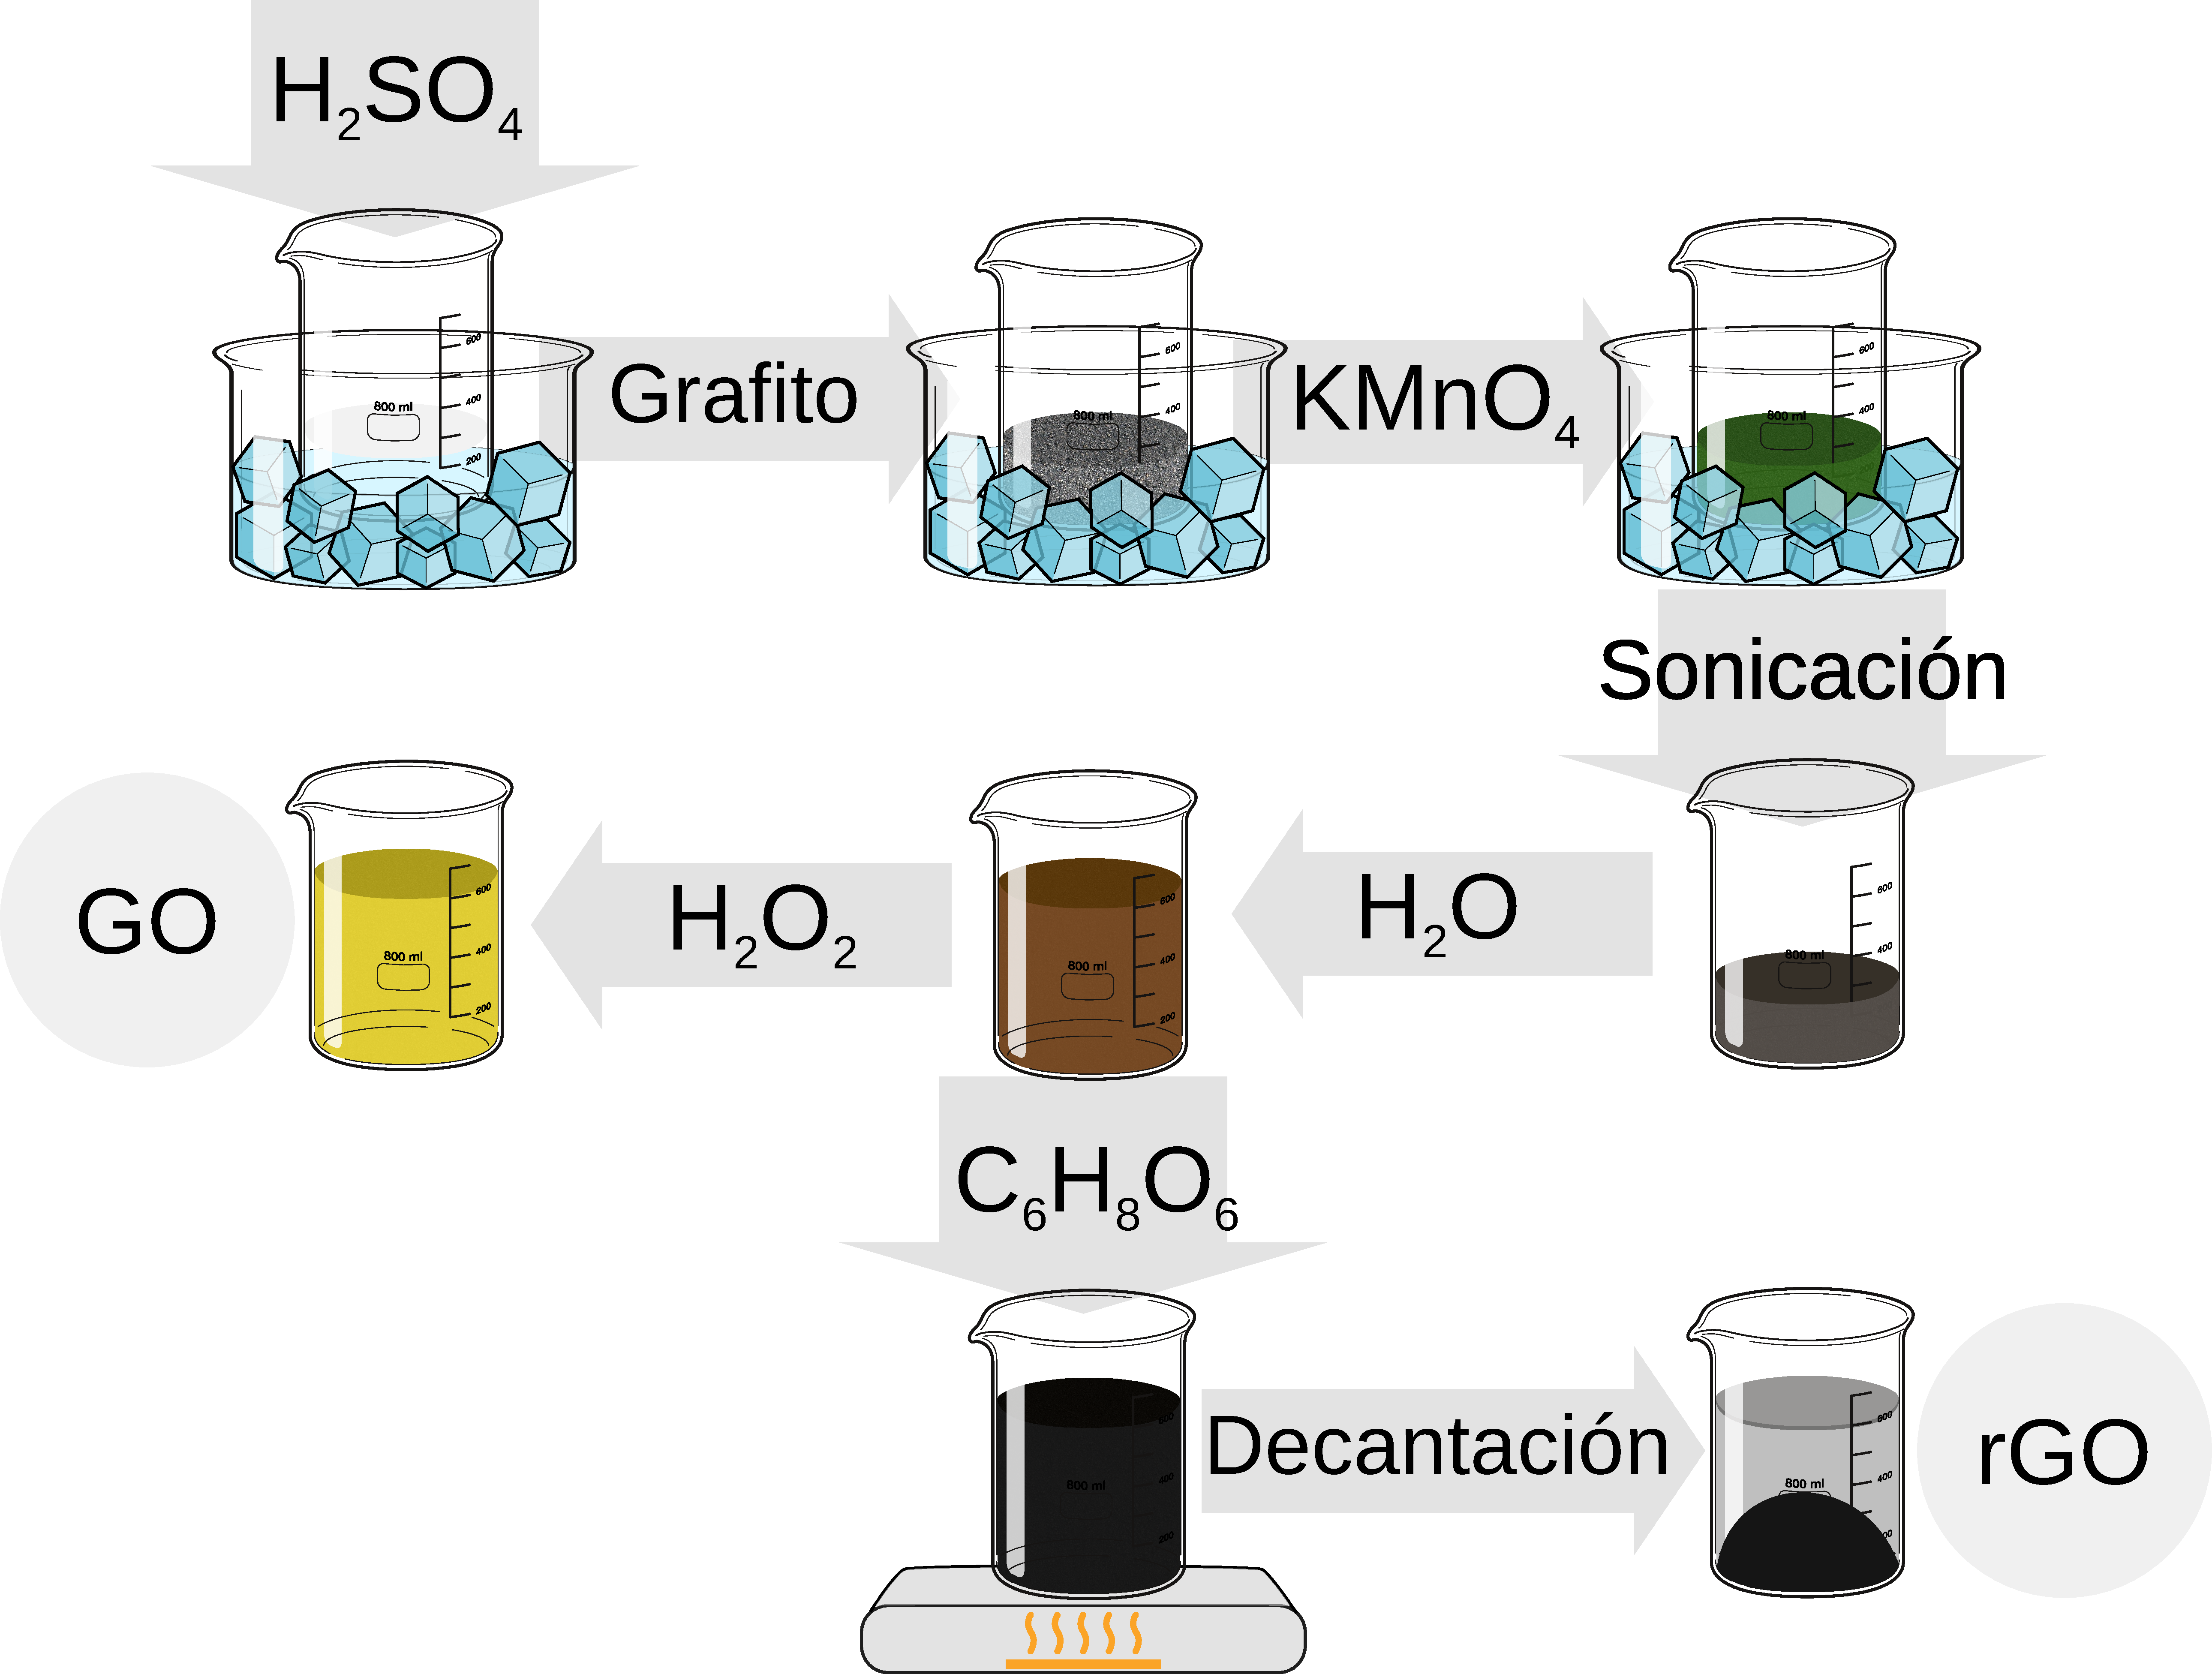
\includegraphics[width=0.8\textwidth]{experimental_method.pdf}
%			}
%			\caption[Método experimental simplicado para la síntesis de óxido de grafeno y óxido reduxido de grafeno]{Método experimental simplificado para la síntesis de óxido de grafeno y óxido reducido de grafeno.}
%		\end{figure}
		\begin{figure}
			\begin{tikzpicture}[]
			\path[ use as bounding box] (-5,-5) rectangle(5,3);
				\only<1->{\begin{scope}
					\clip[] (-3.5, 1.5)	circle(\clipradius);
					\node at (0, -1) {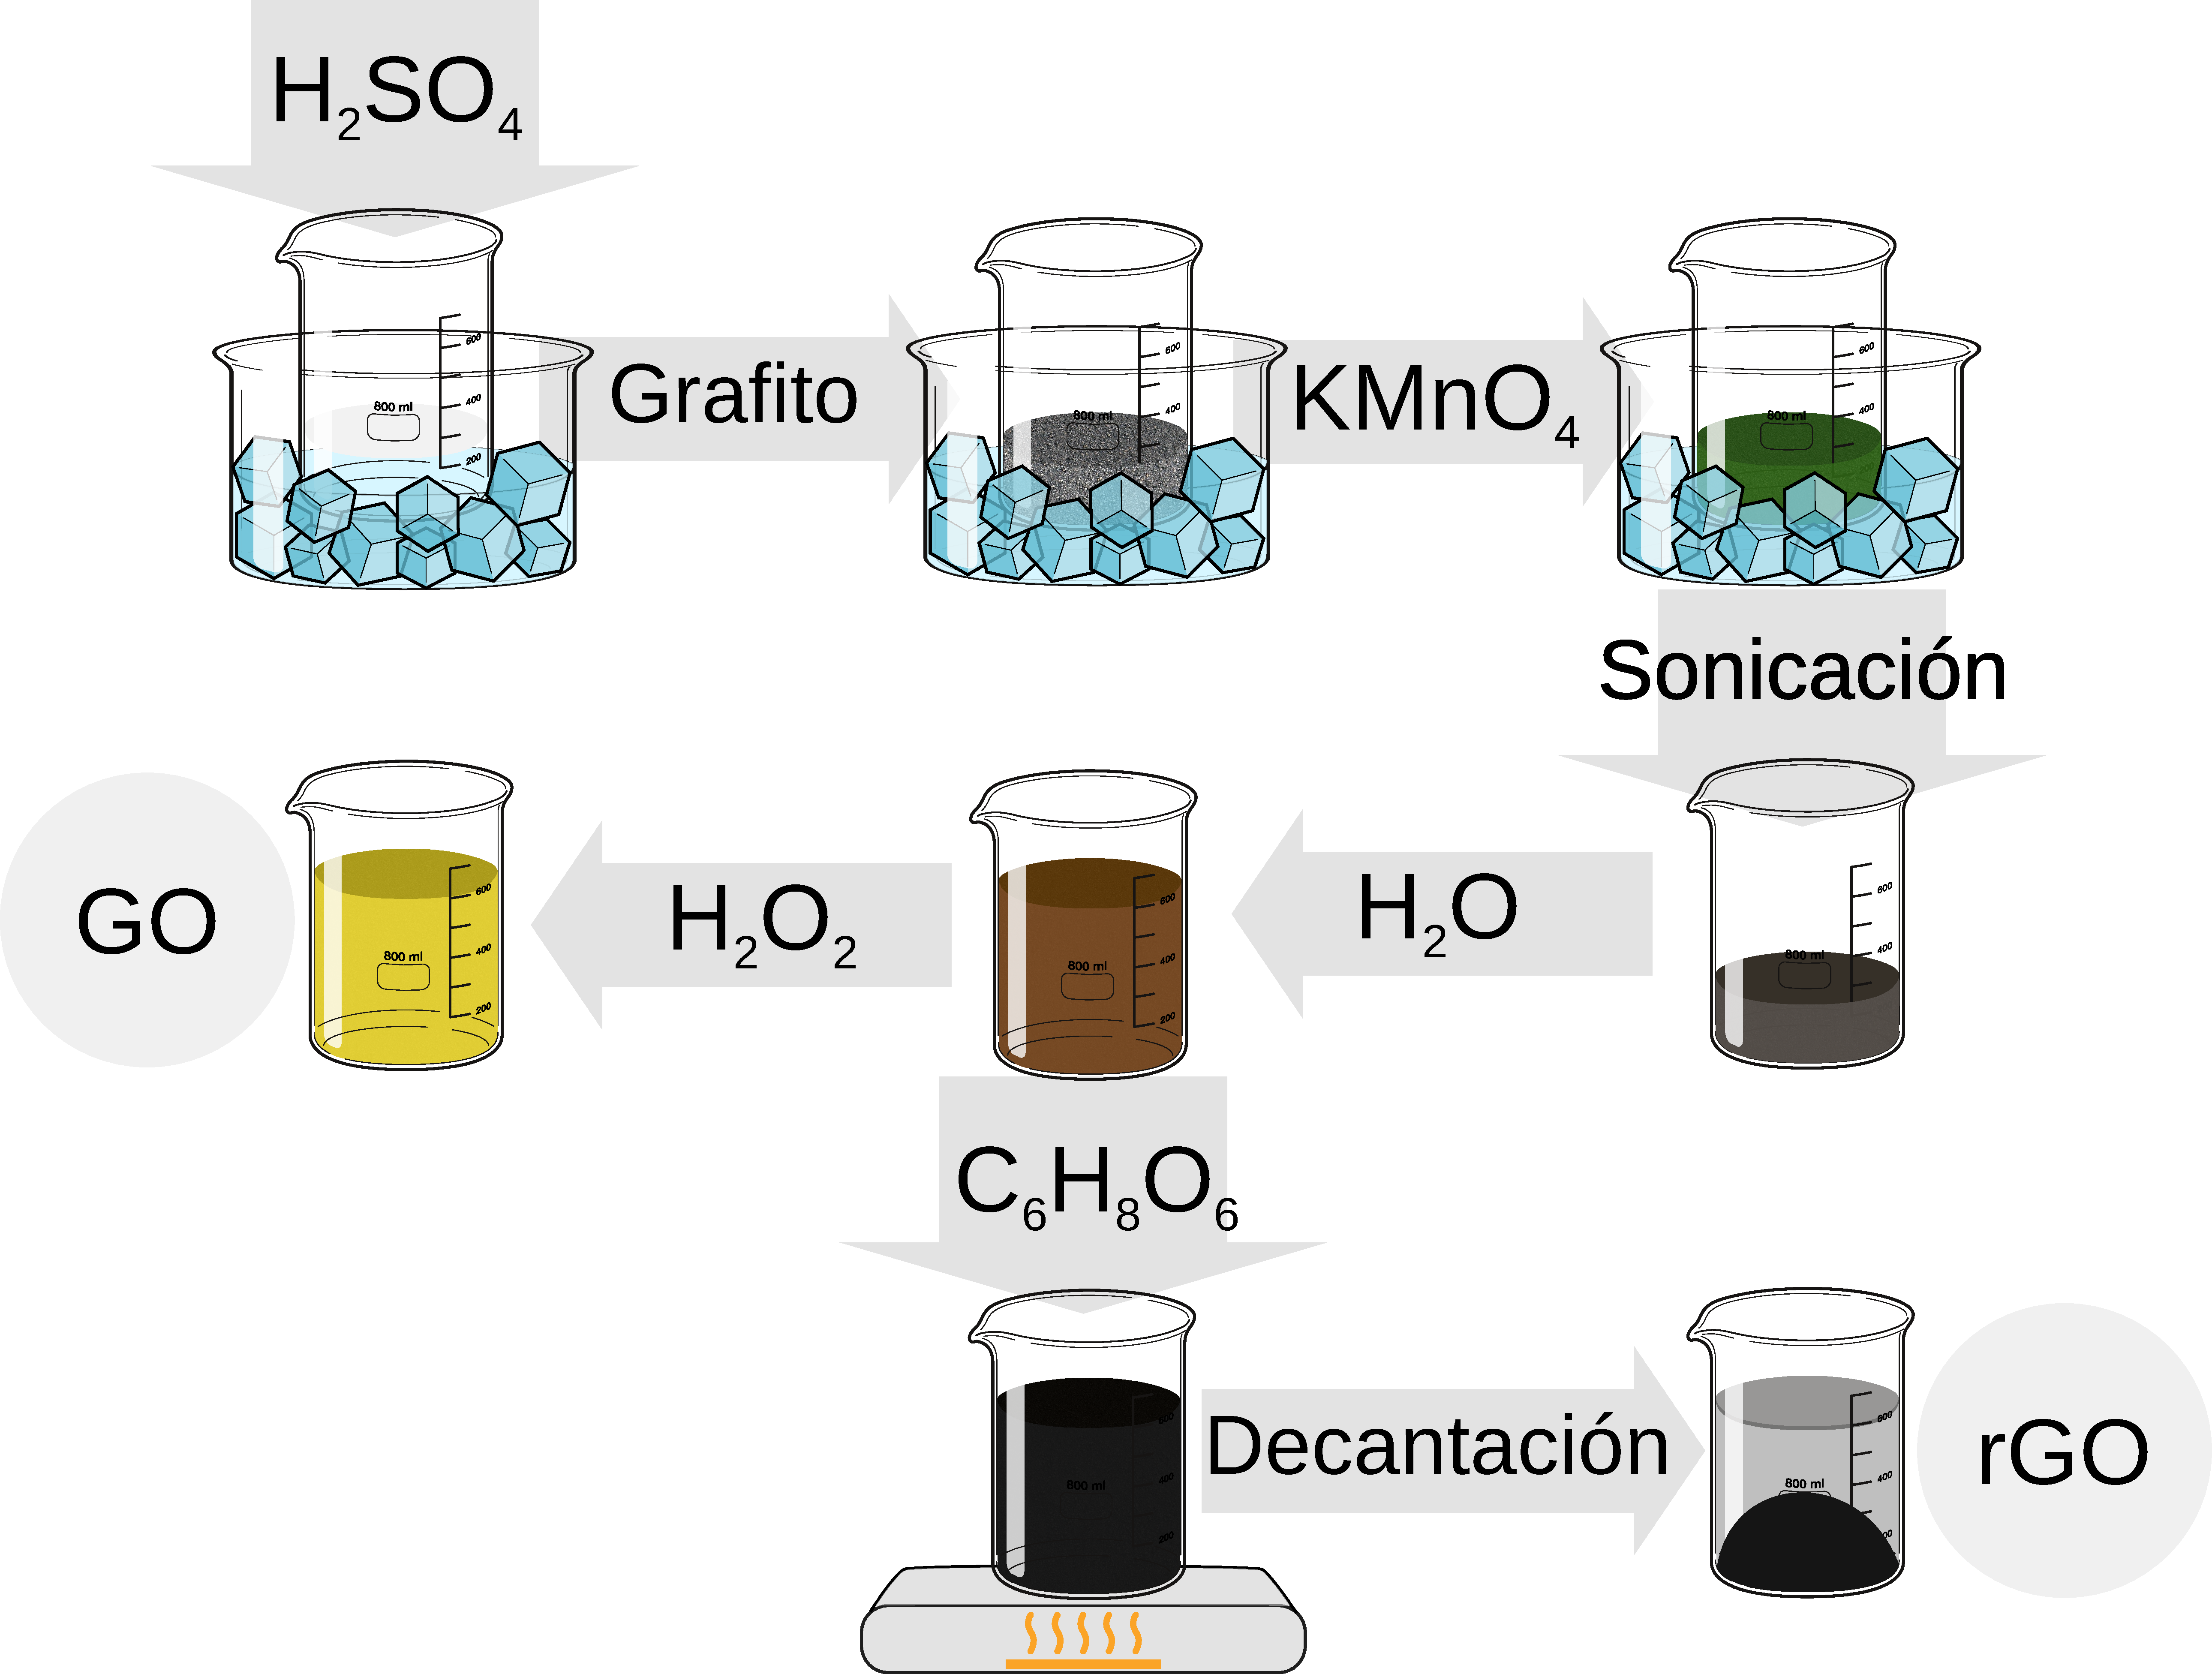
\includegraphics[width=\textwidth]{experimental_method.pdf}};
				\end{scope}}
				\only<2->{\begin{scope}
					\clip[] (0, 1.5)	circle(\clipradius);
					\node at (0, -1) {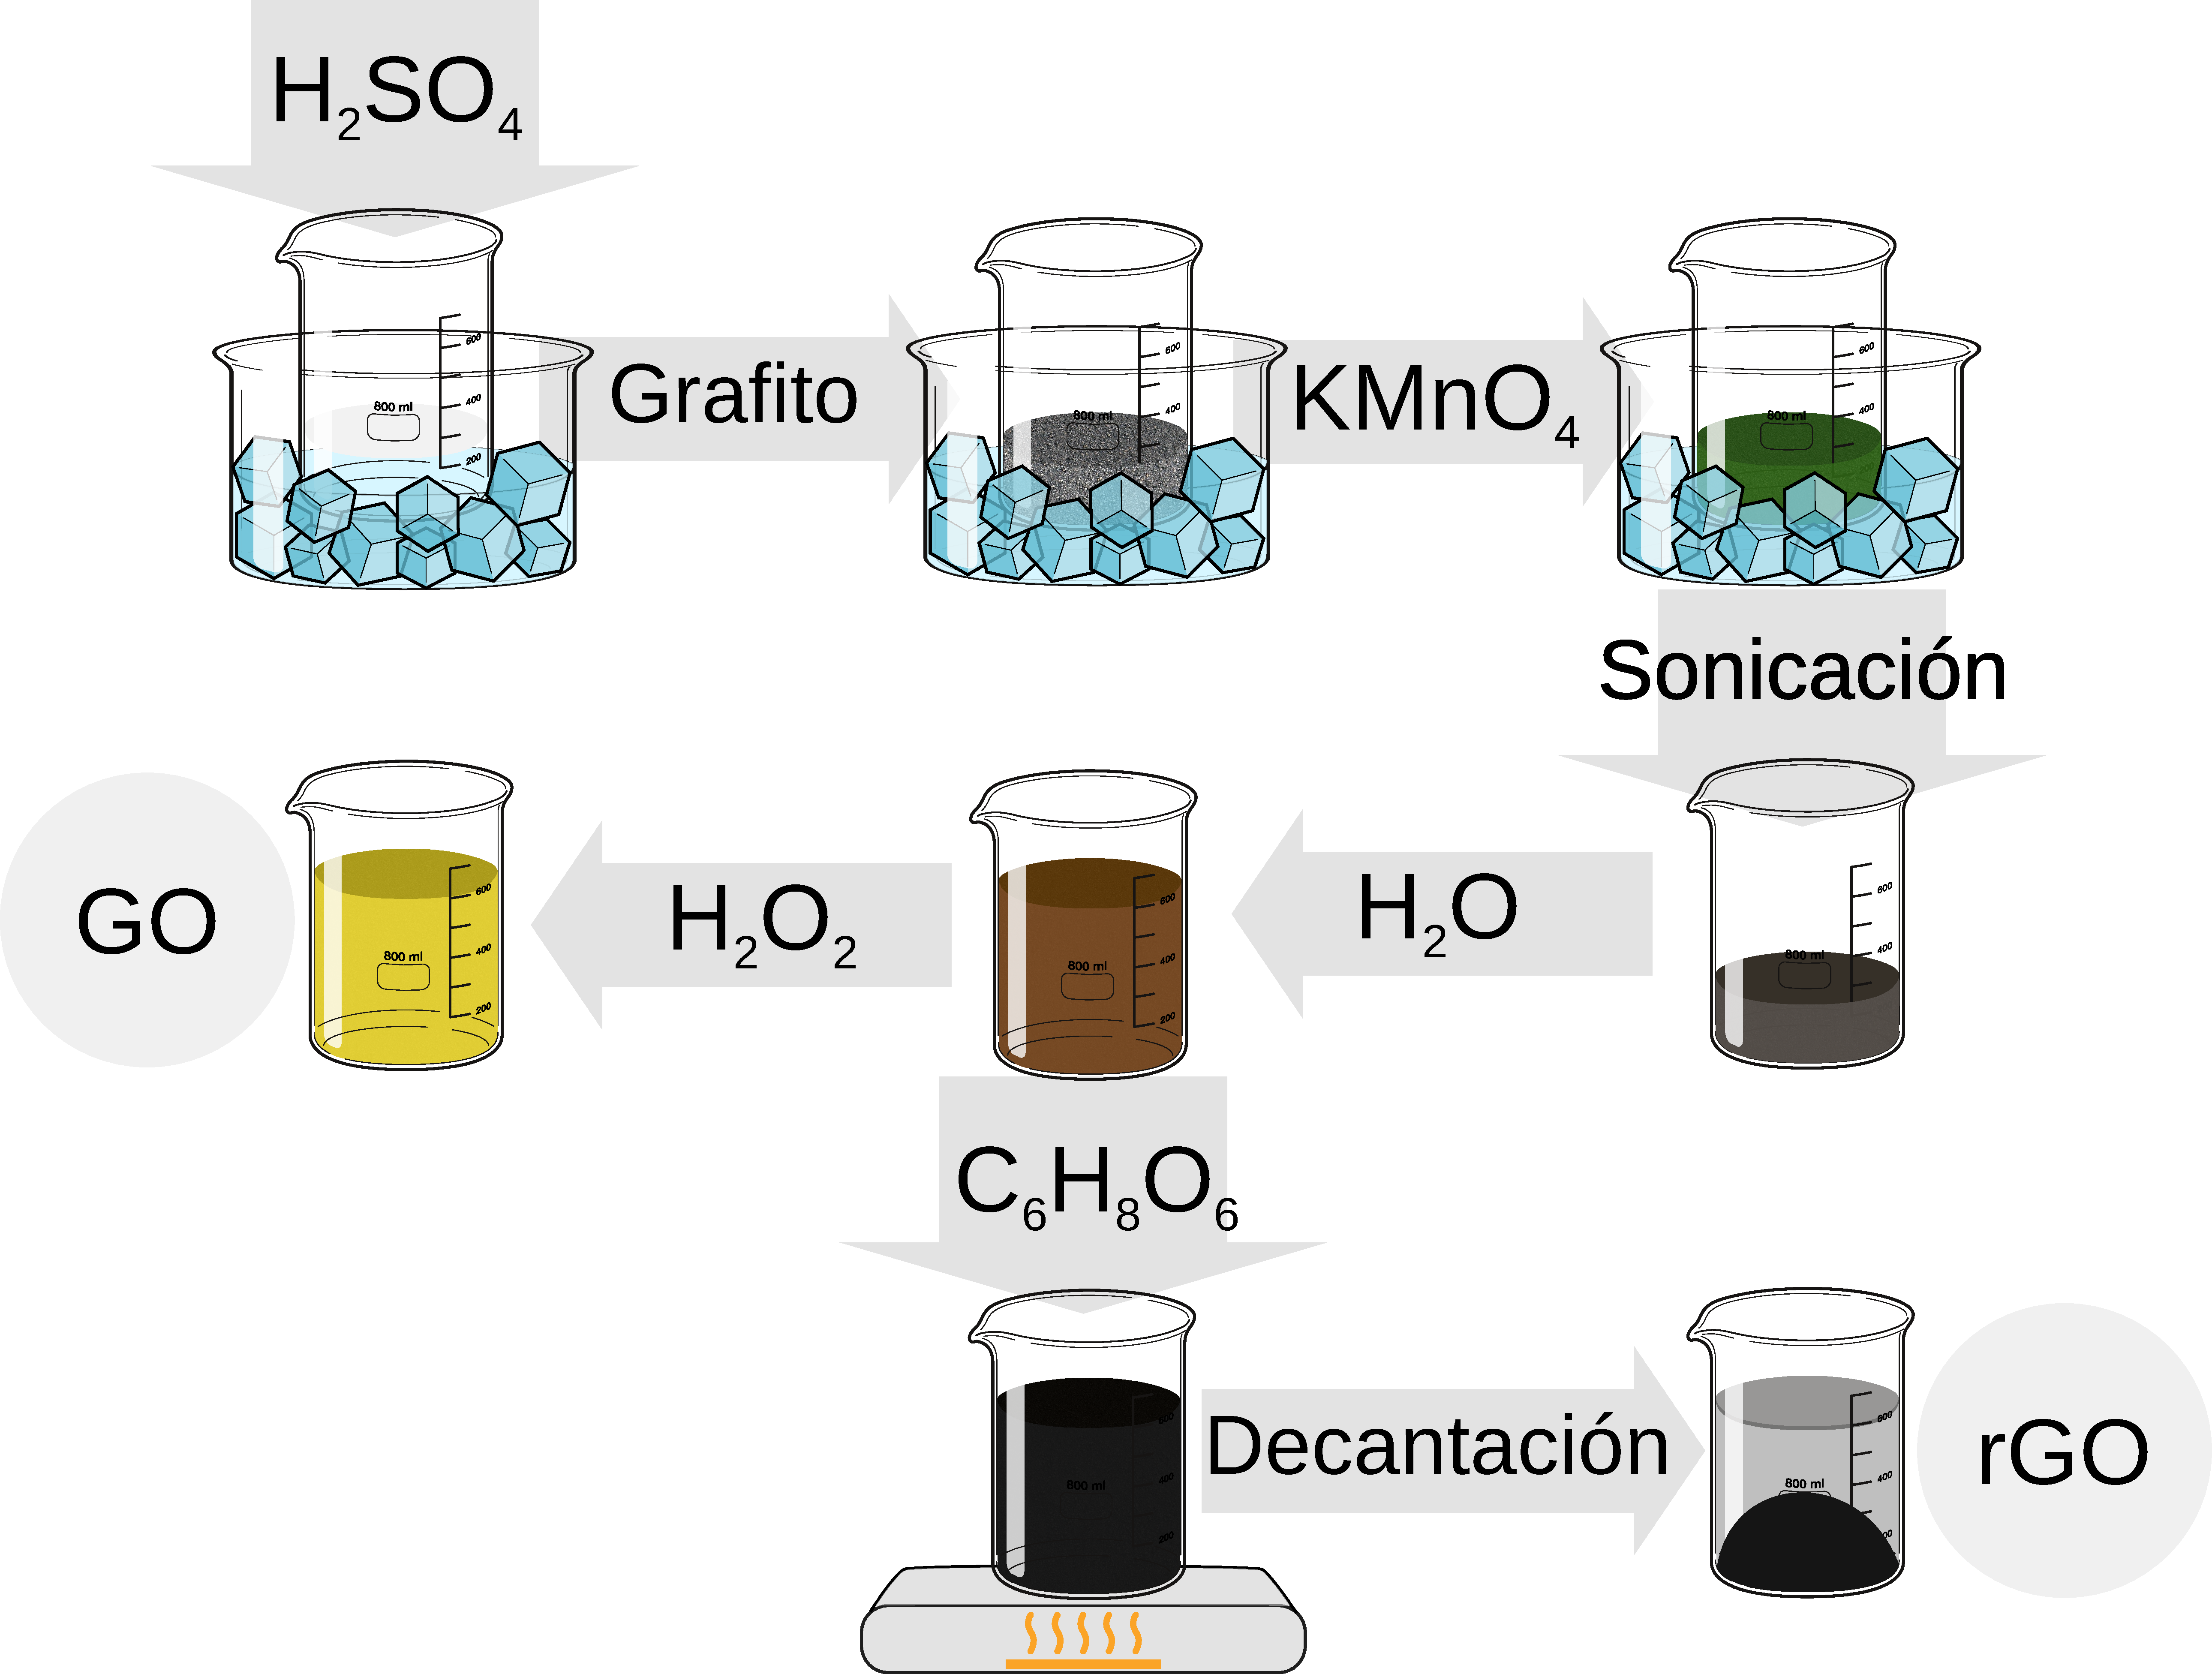
\includegraphics[width=\textwidth]{experimental_method.pdf}};
					\end{scope}}
				\only<3->{\begin{scope}
					\node[draw] at (5,1.5) {\ce{Mn2O7}};
					\node[scale=1] at (5,1) {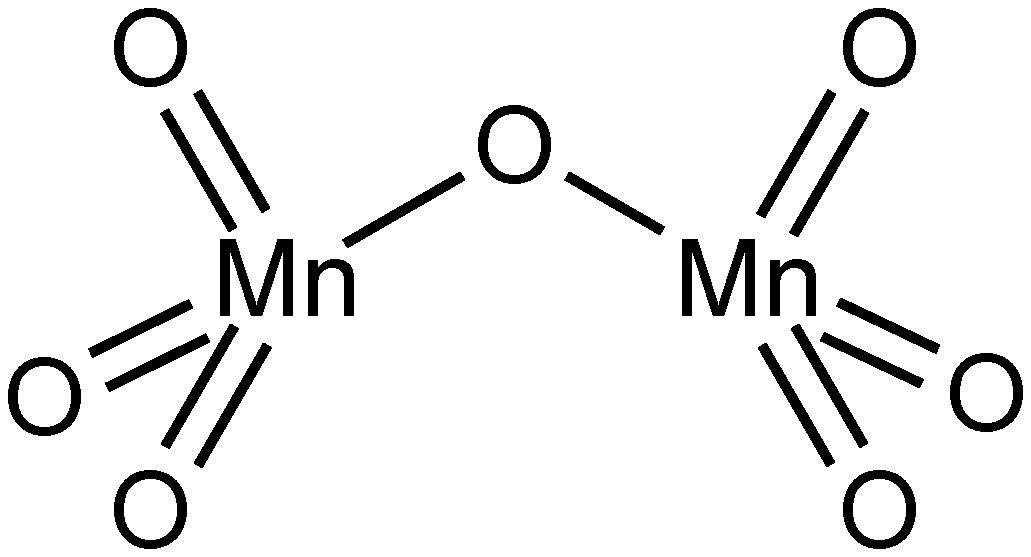
\includegraphics[width=1cm]{Mn2O7.pdf}};
					\clip[] (3.5, 1.5)	circle(\clipradius);
					\node at (0, -1) {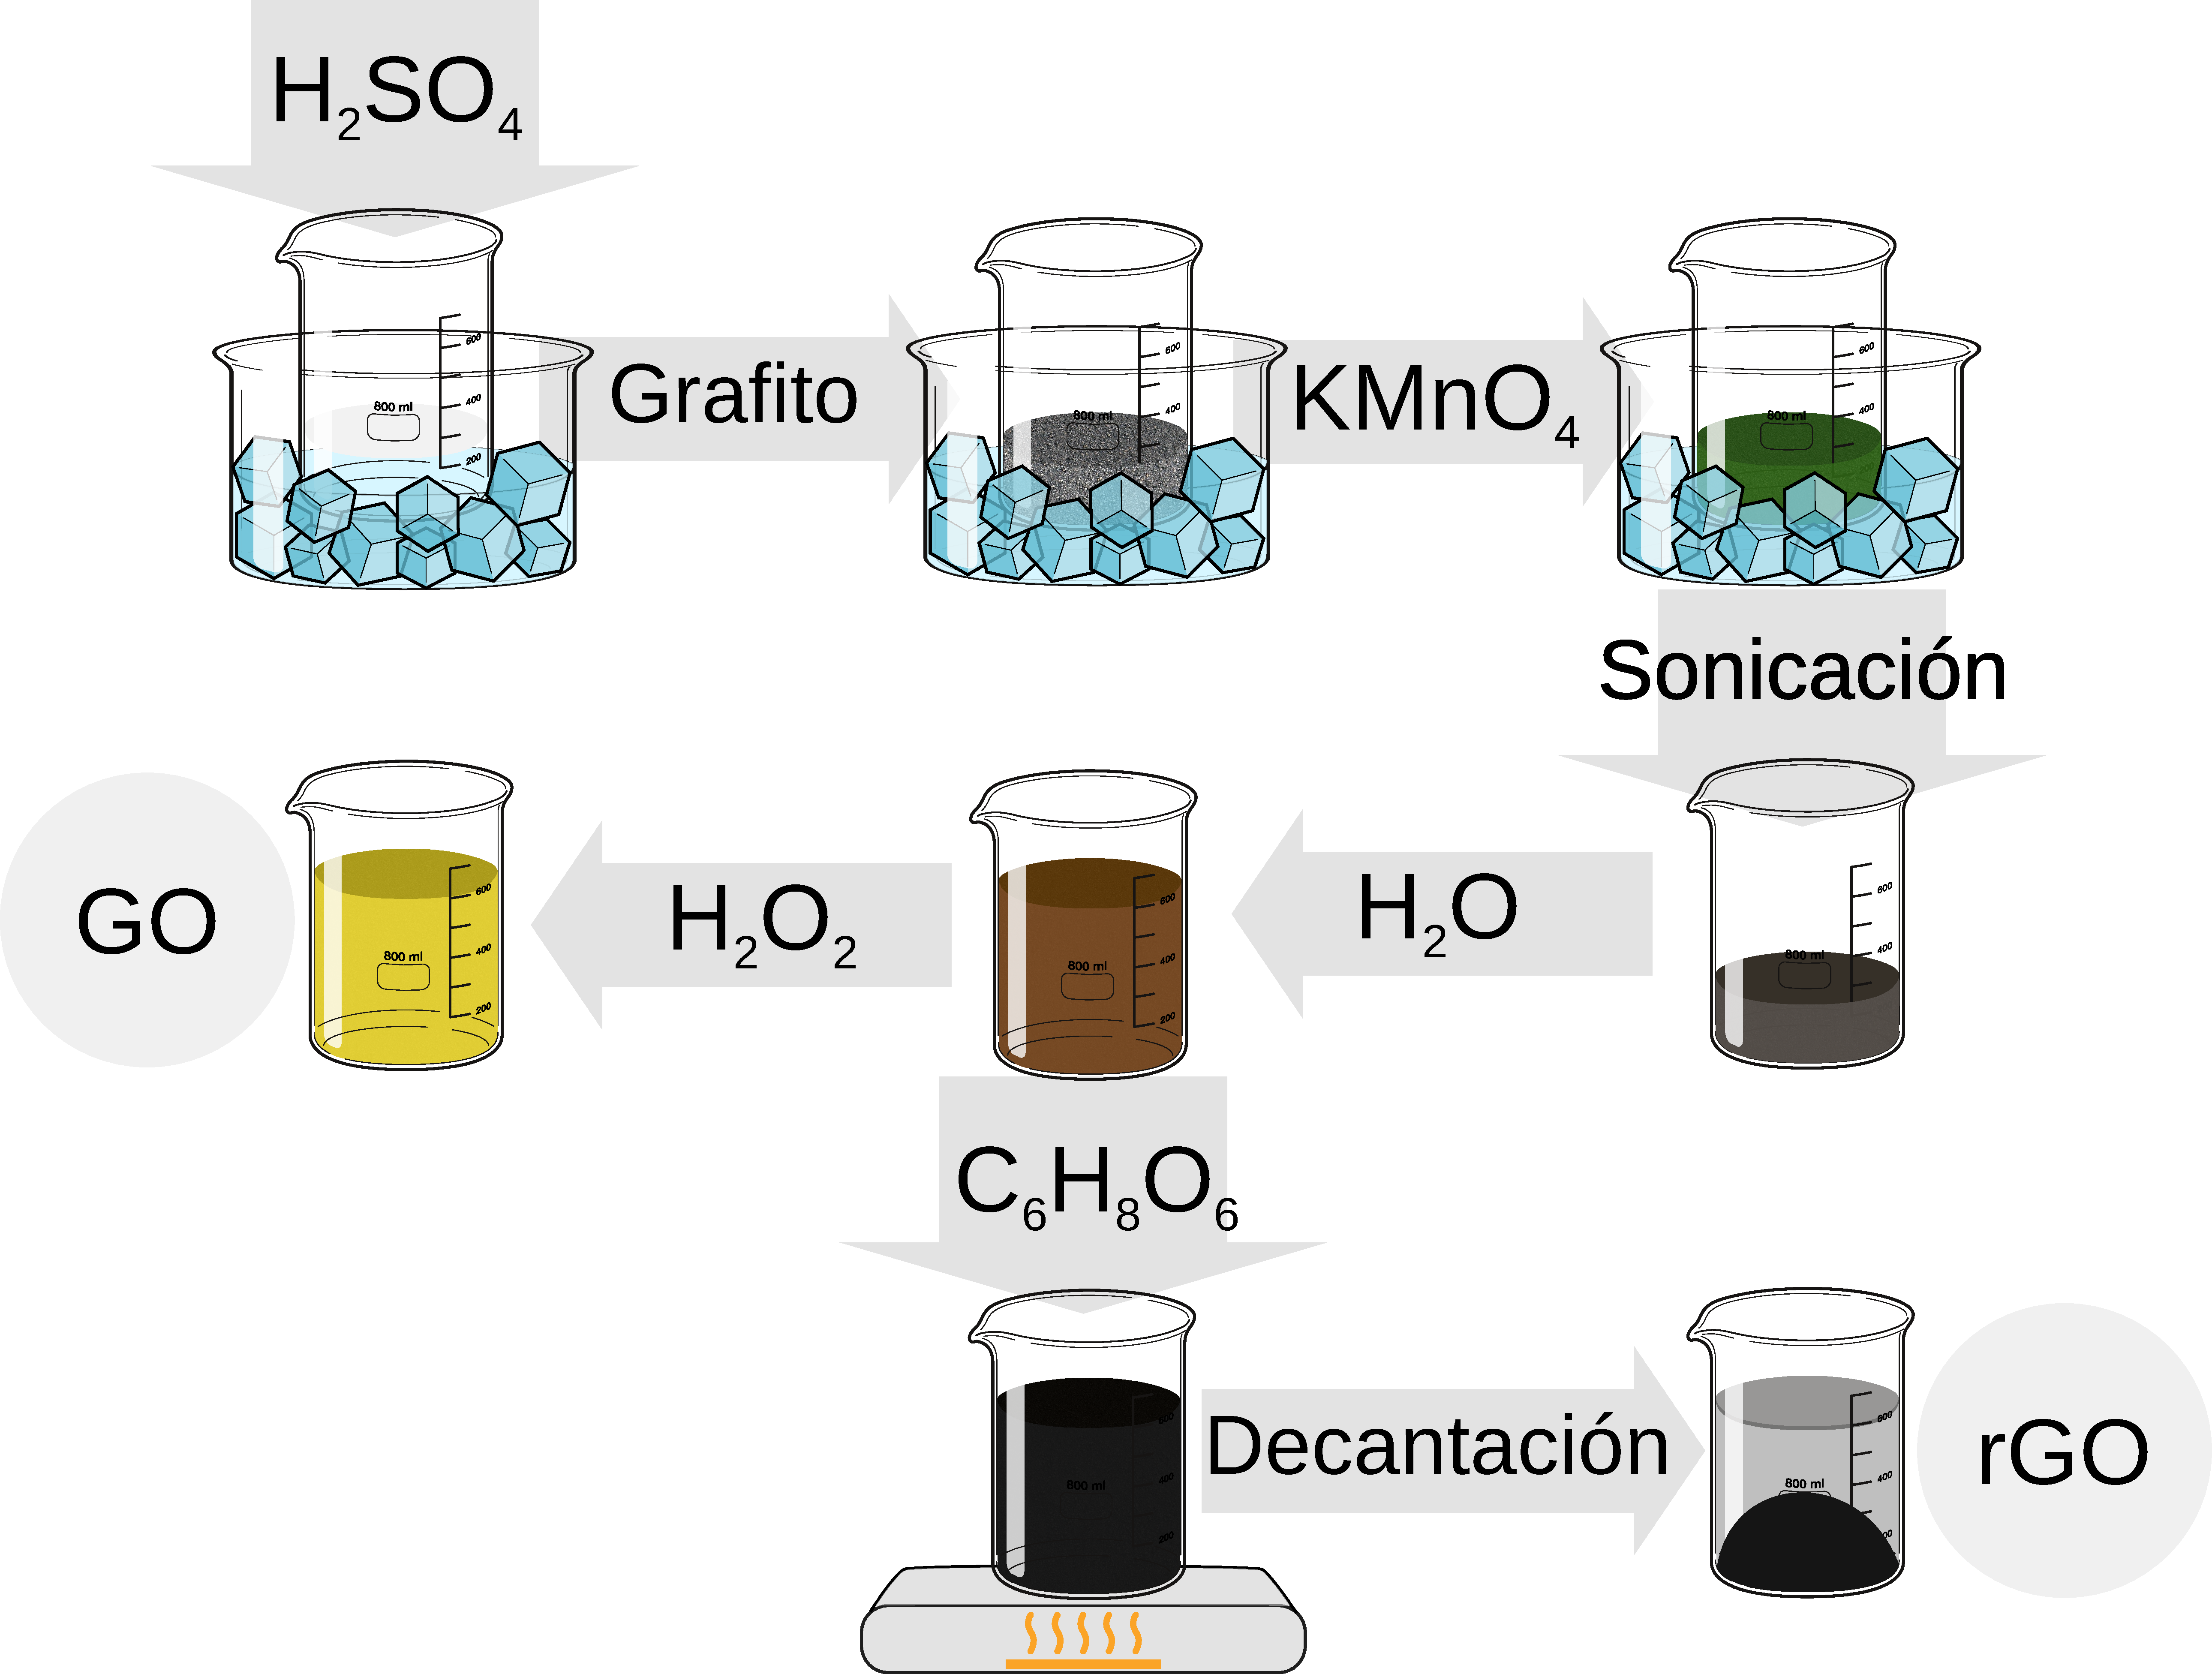
\includegraphics[width=\textwidth]{experimental_method.pdf}};
					\end{scope}}
				\only<4->{\begin{scope}
					\clip[] (3.5, -1) circle(\clipradius);
					\node at (0, -1) {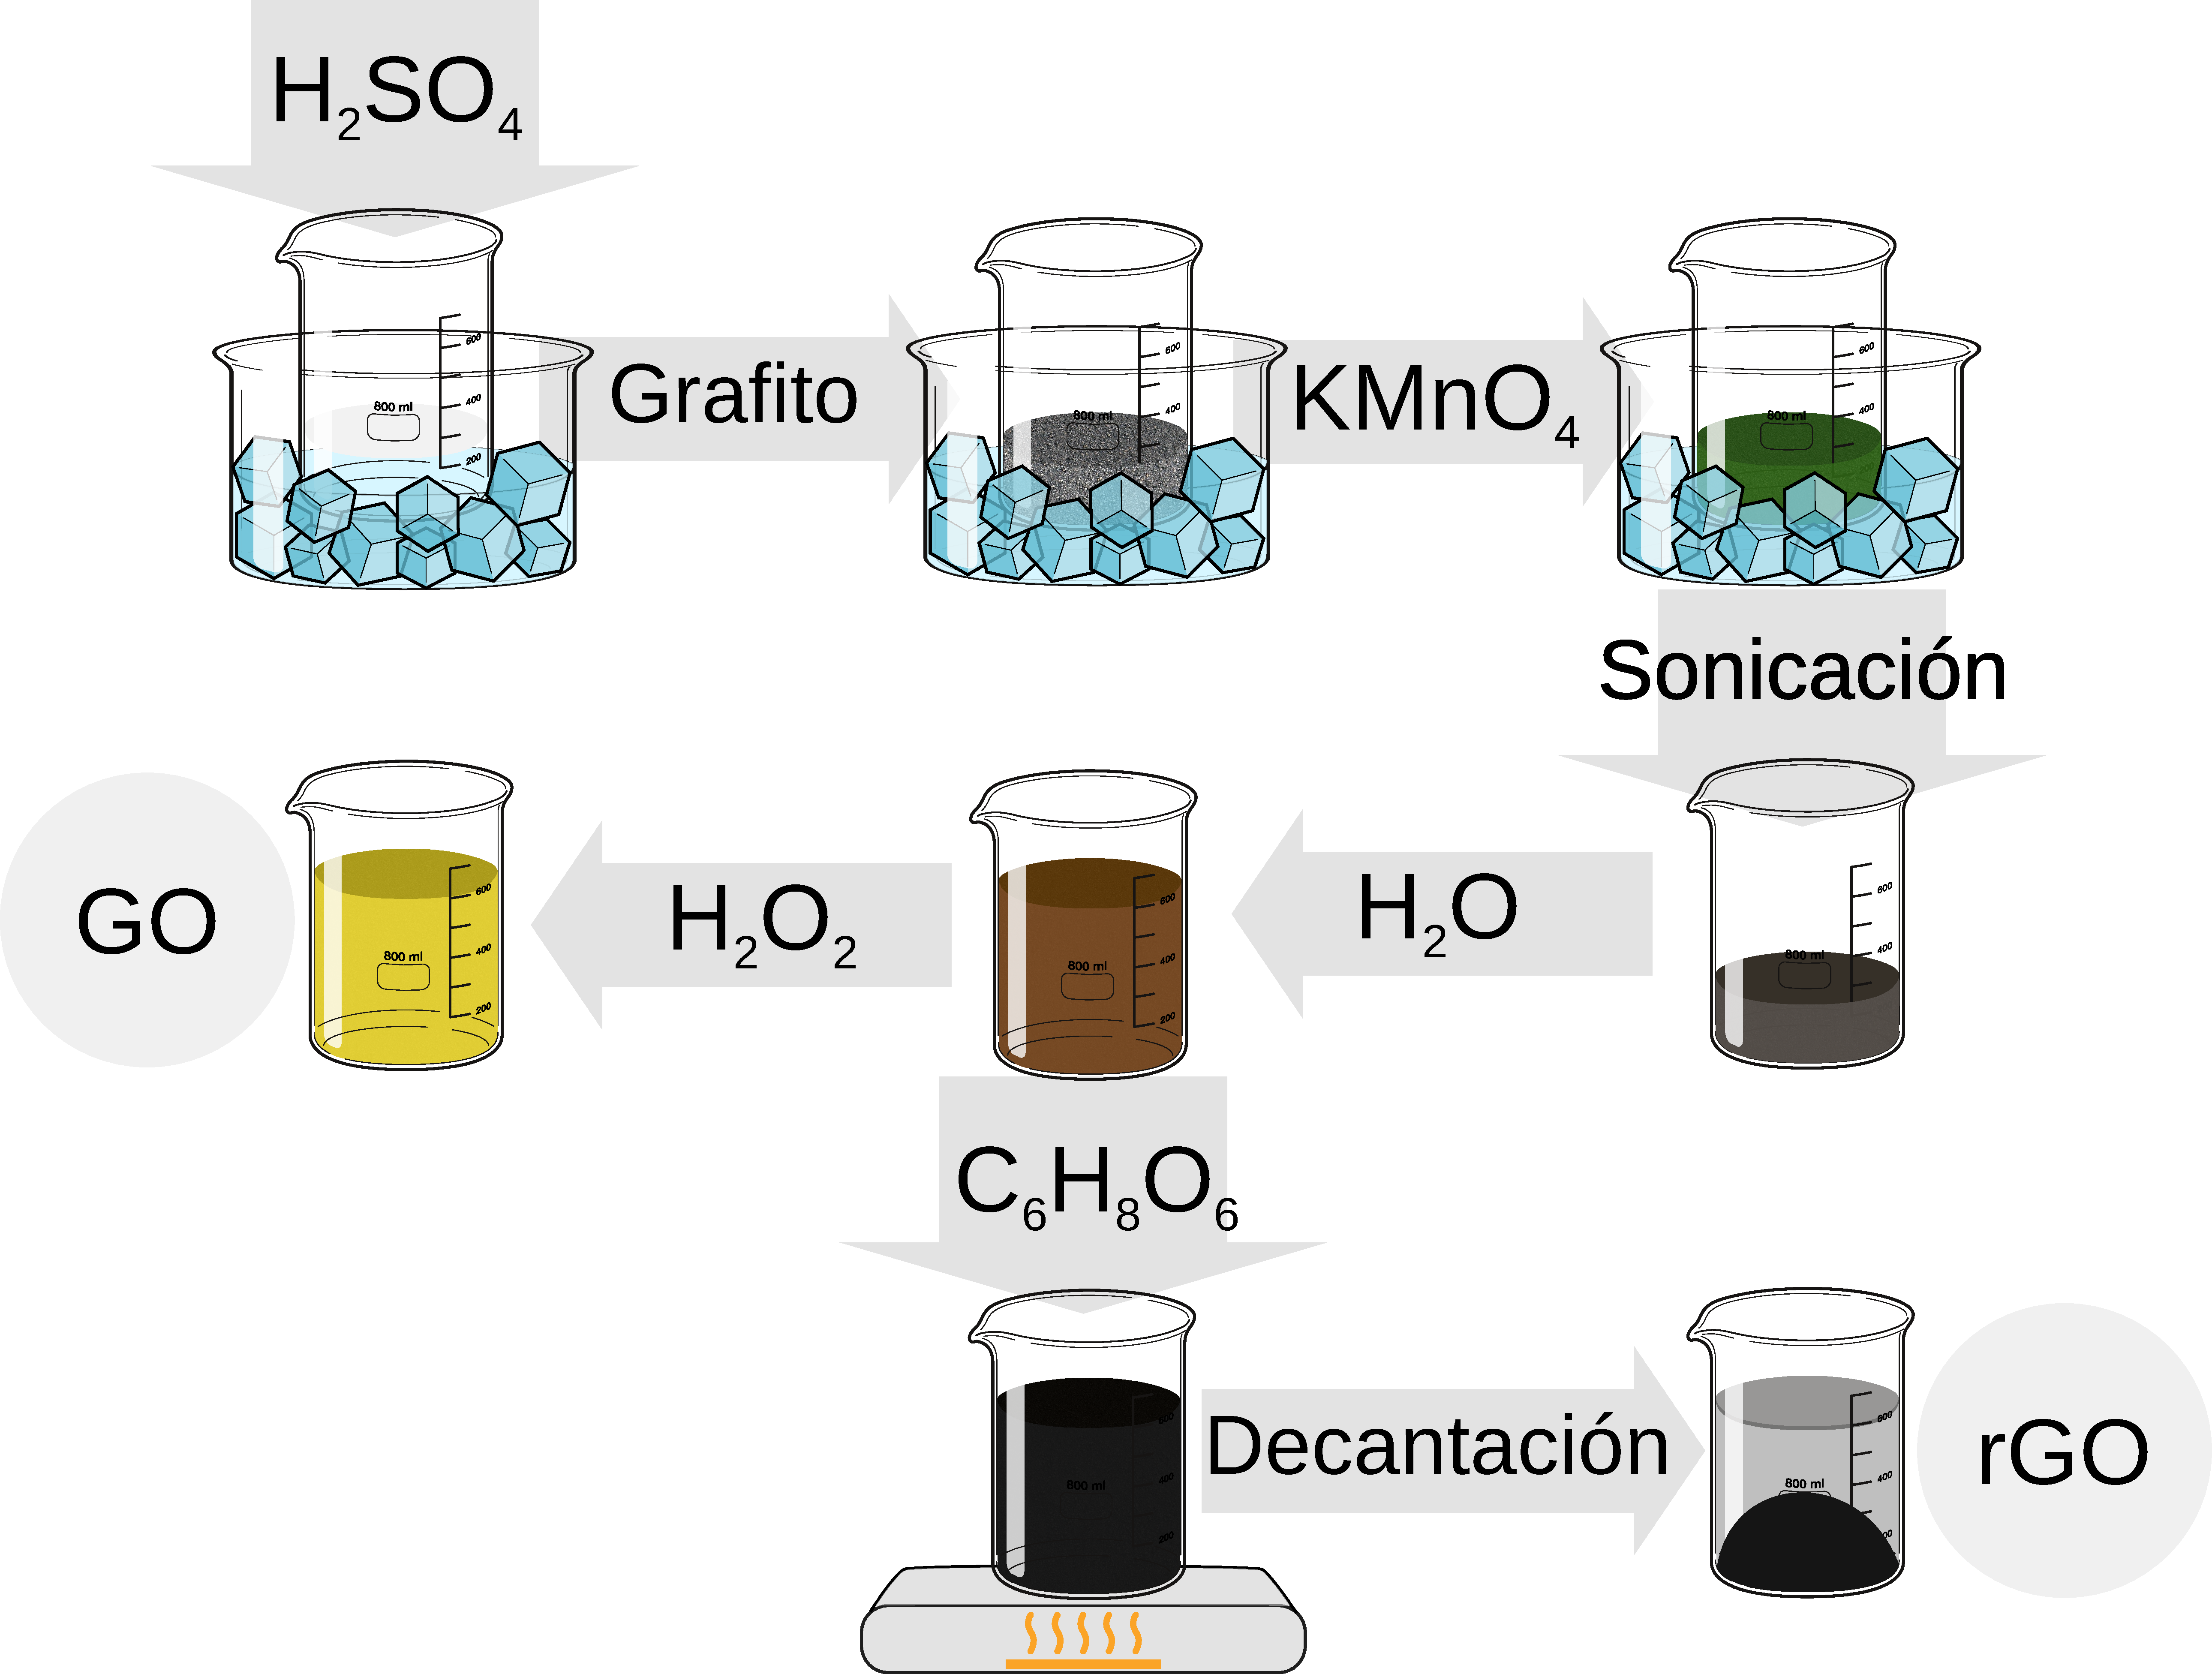
\includegraphics[width=\textwidth]{experimental_method.pdf}};
					\end{scope}}
				\only<5->{\begin{scope}
					\clip[] ( 0, -1) circle(\clipradius);
					\node at (0, -1) {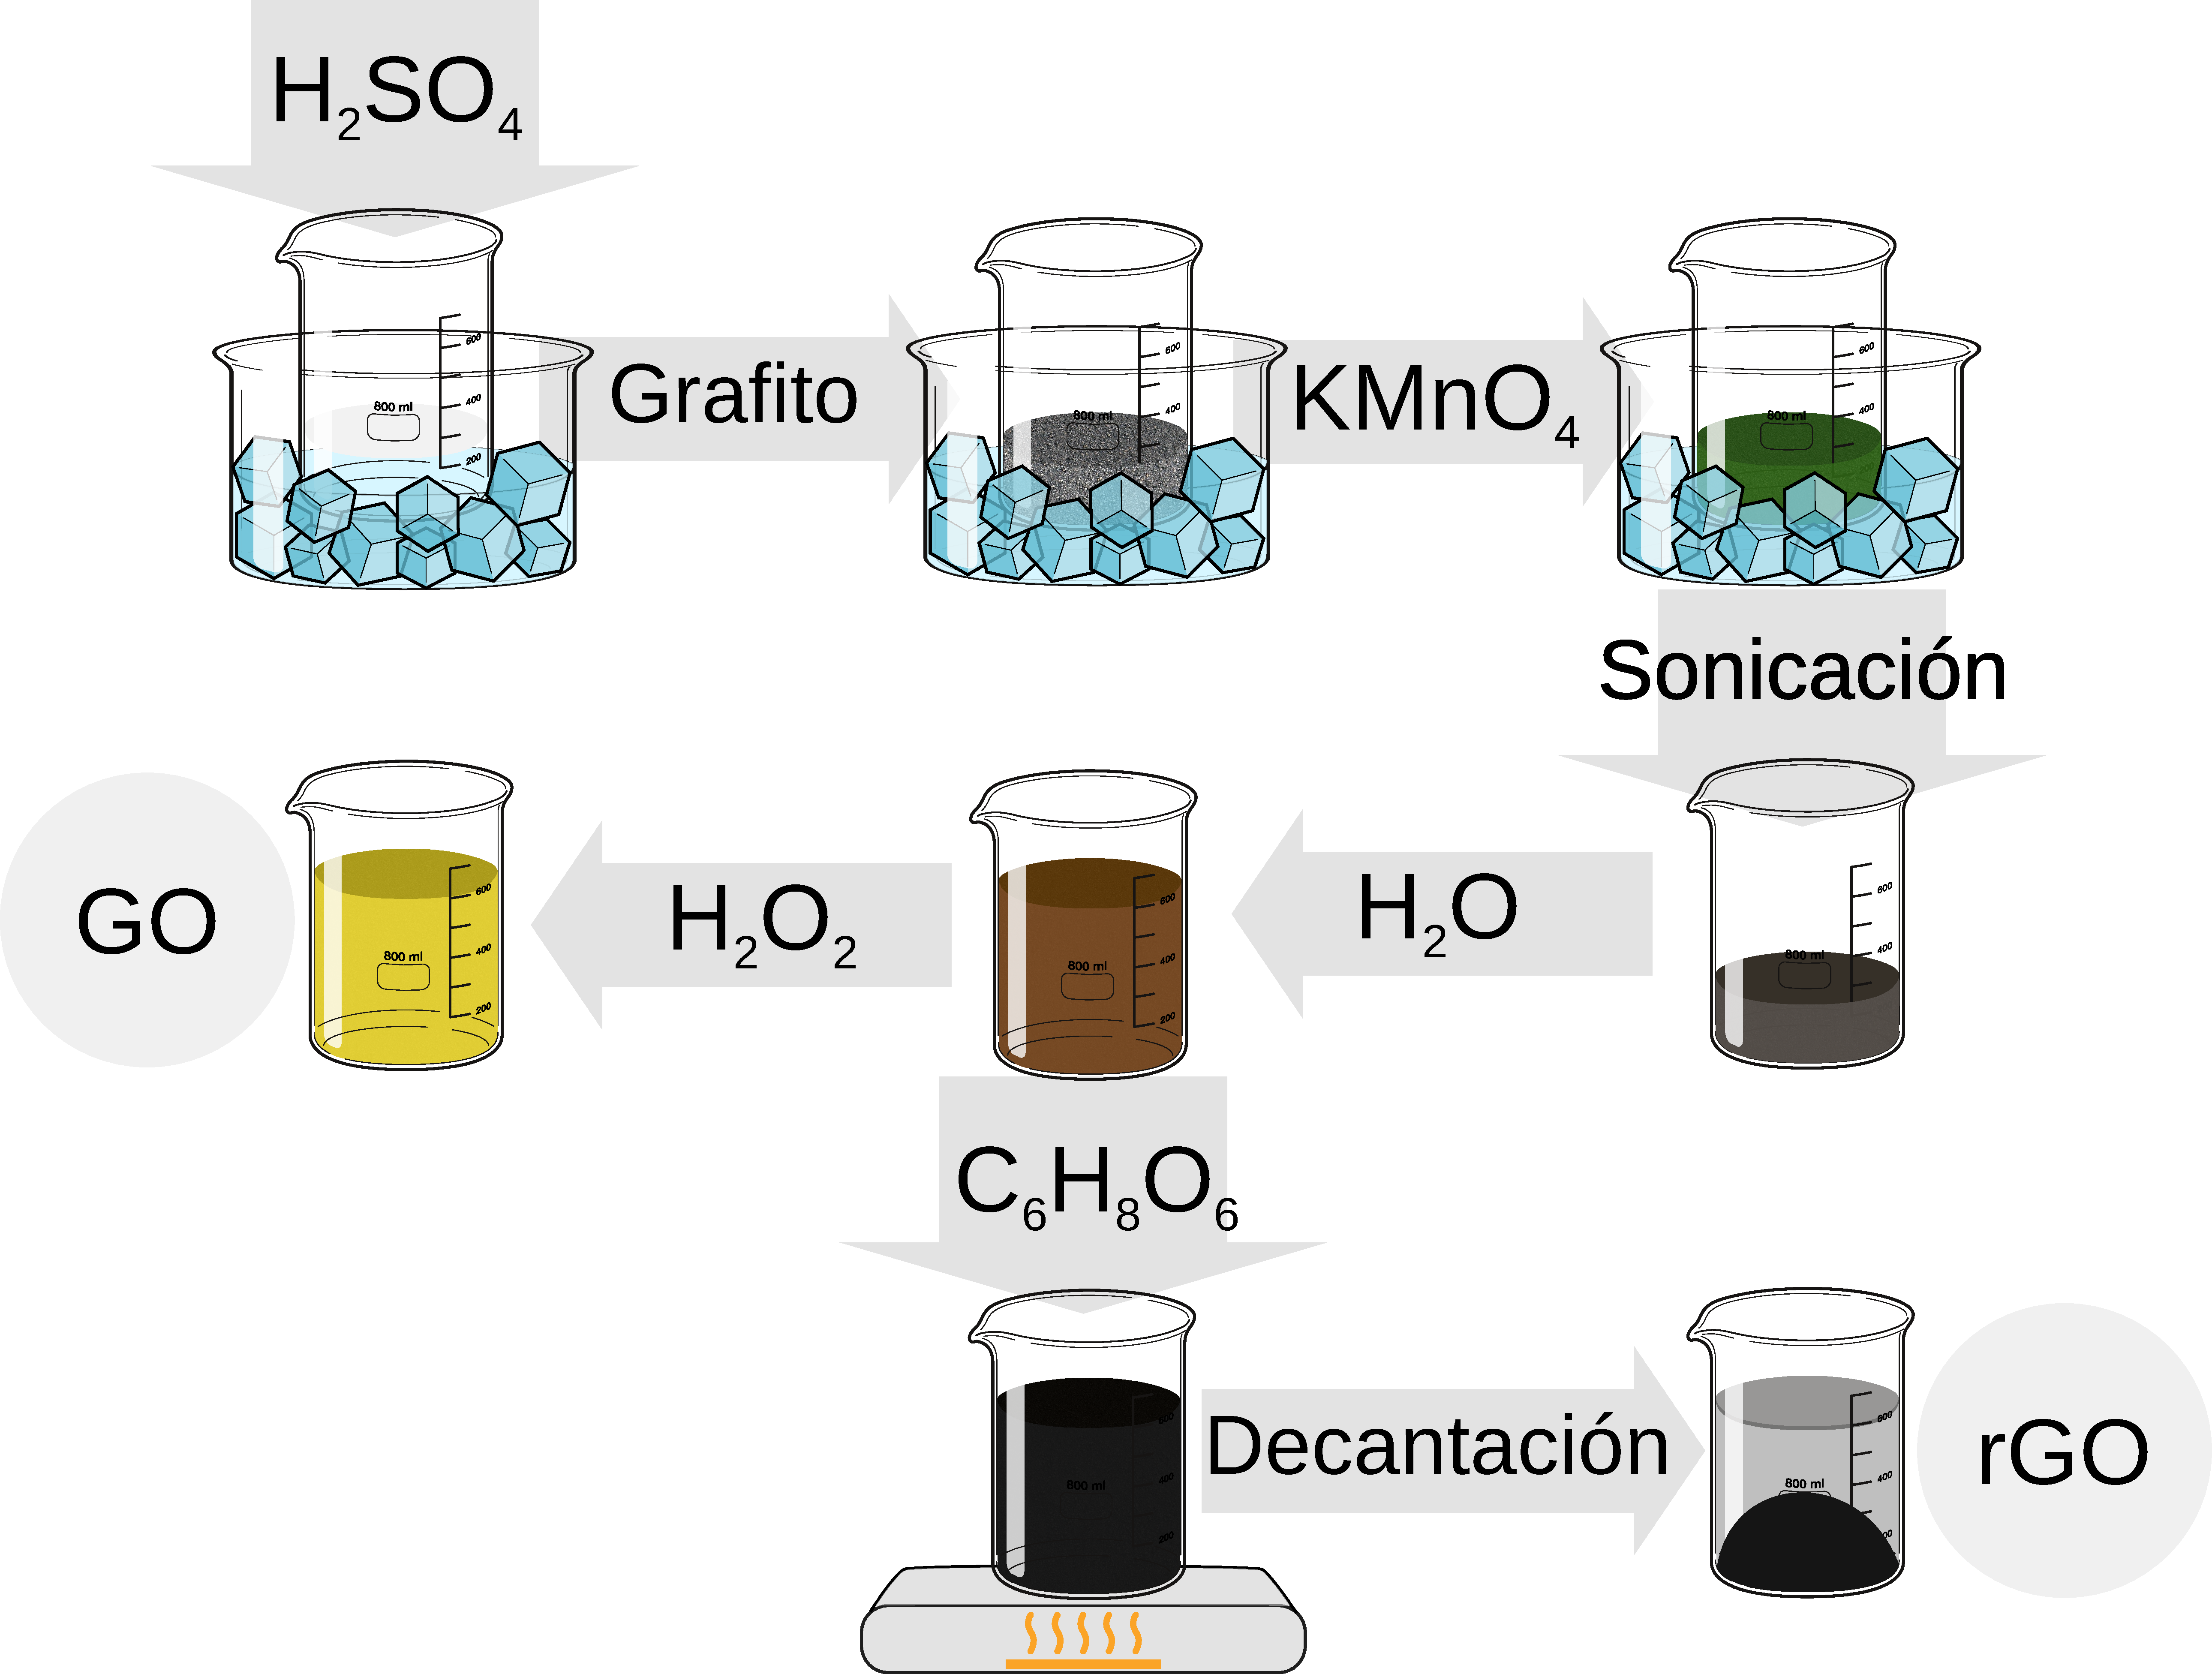
\includegraphics[width=\textwidth]{experimental_method.pdf}};
				\end{scope}}
				\only<6->{\begin{scope}
					\clip[] (-3.5, -1) circle(\clipradius);
					\node at (0, -1) {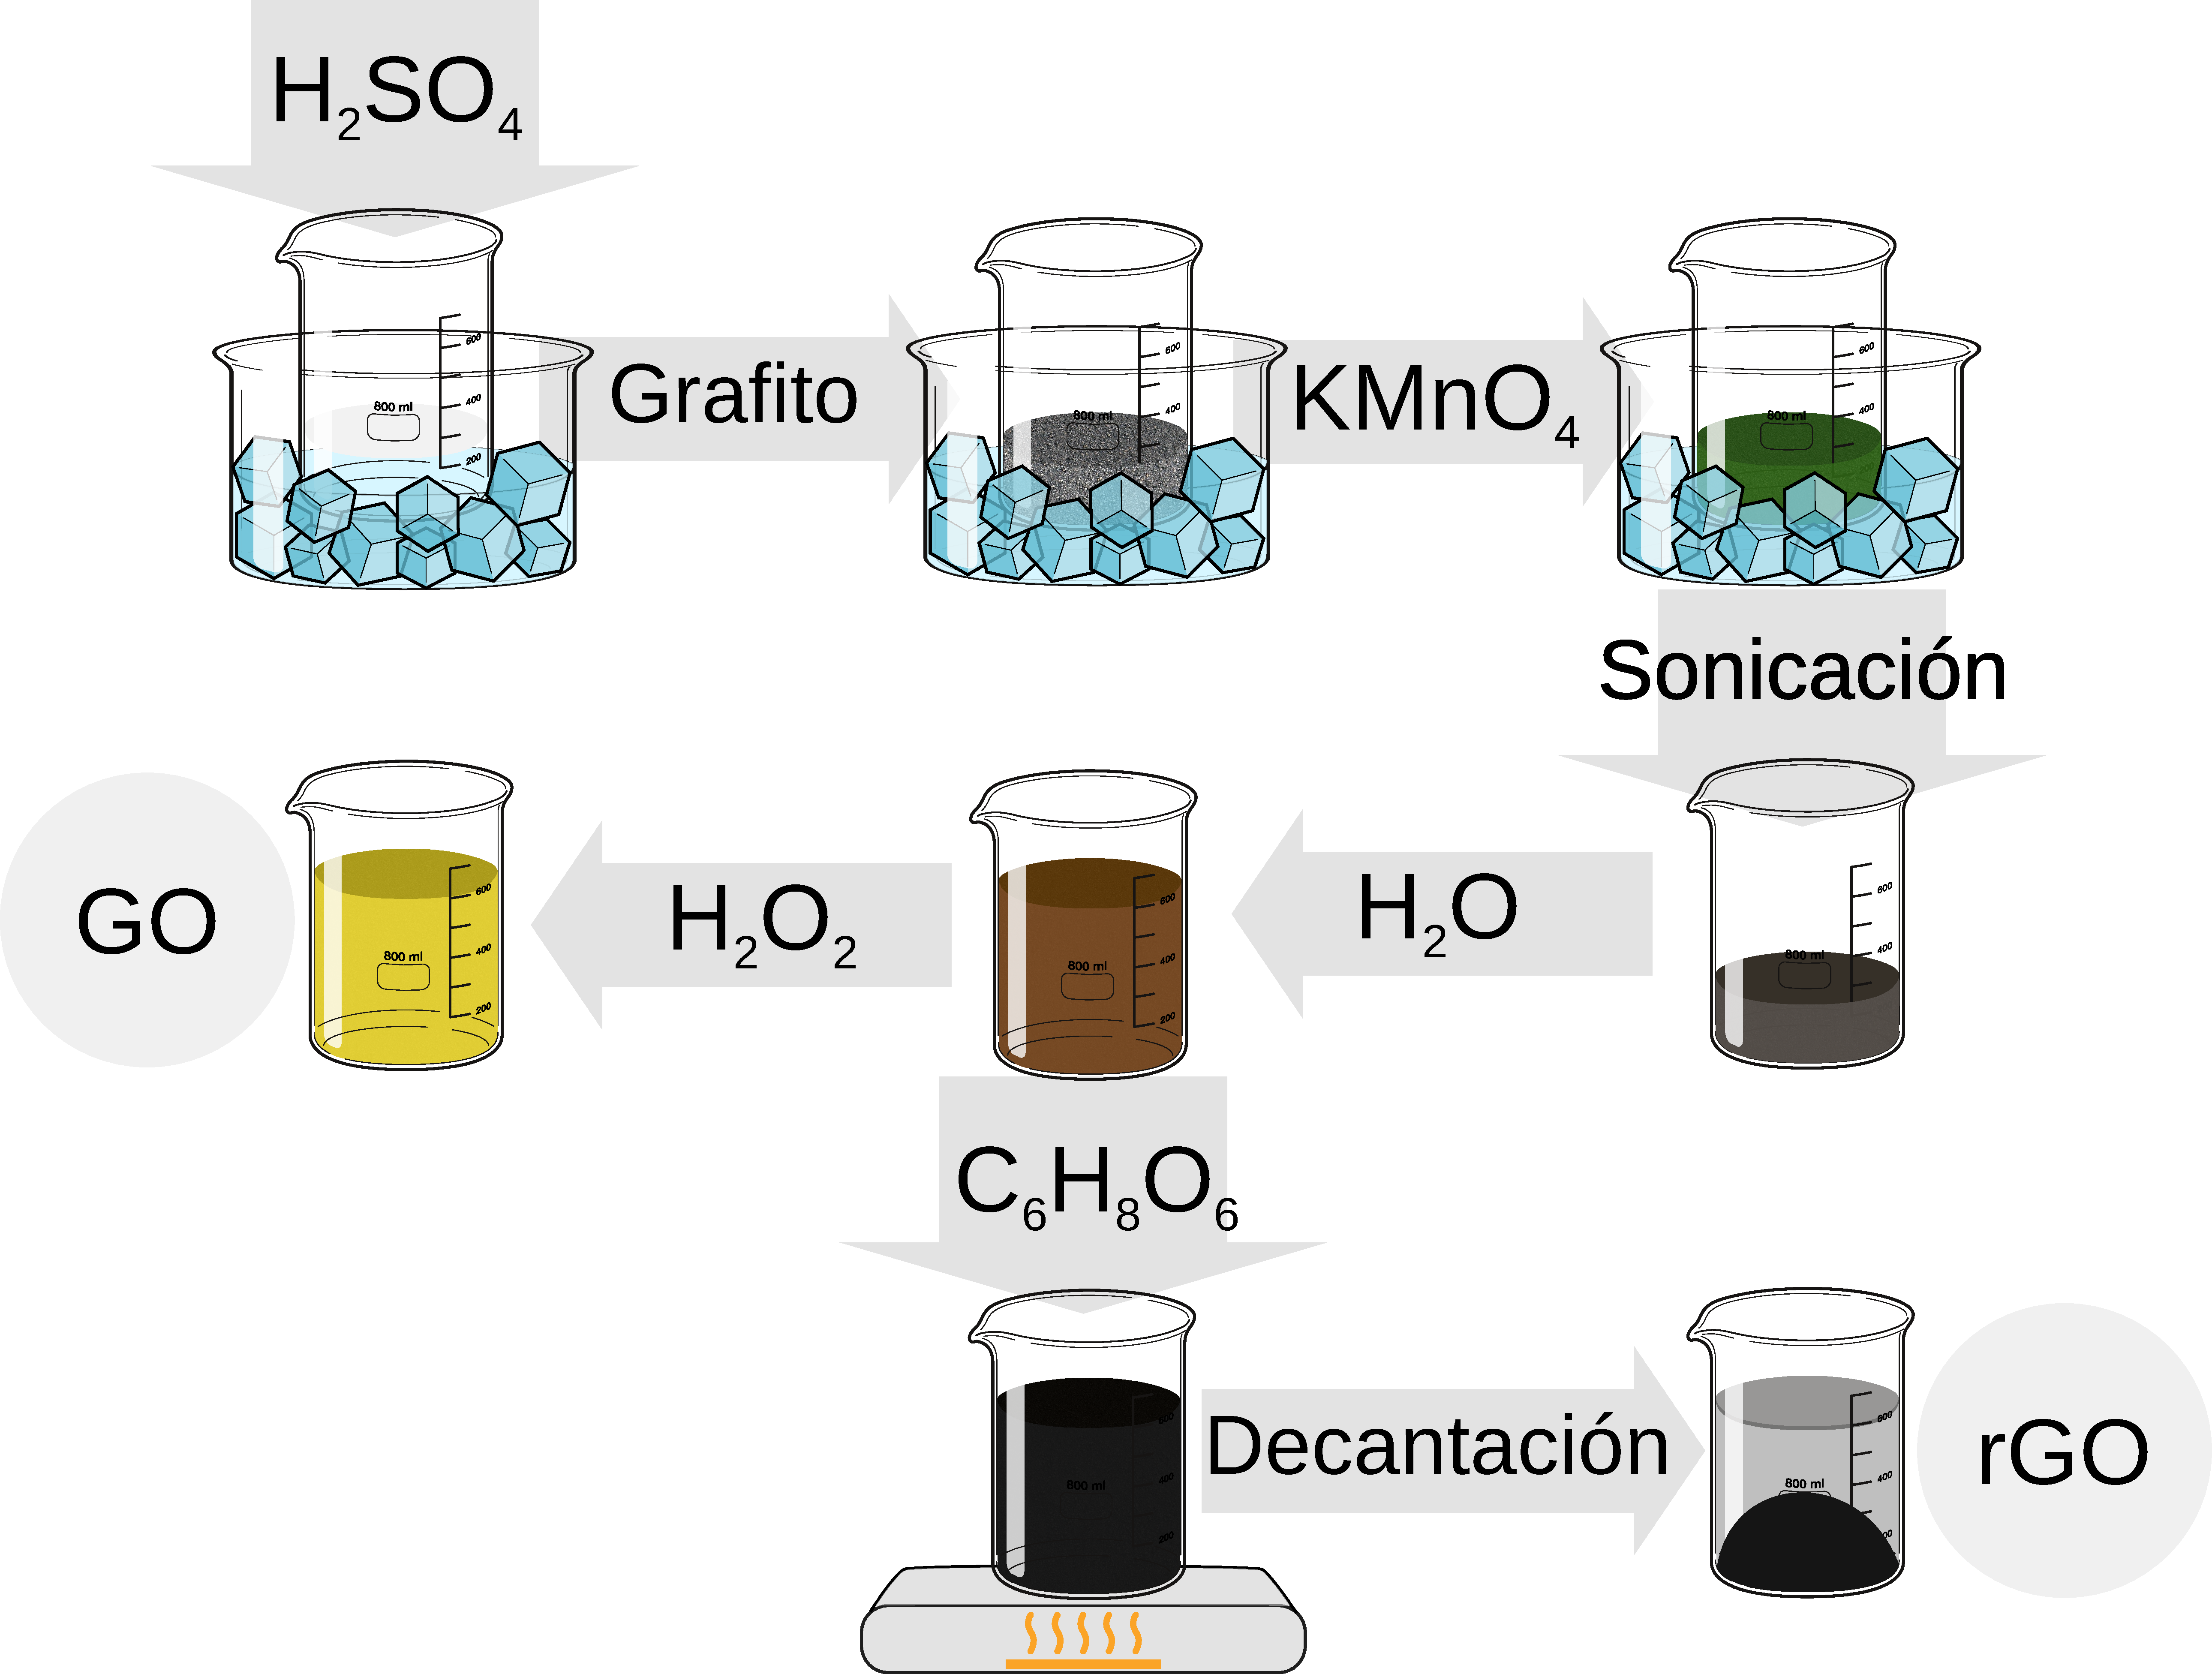
\includegraphics[width=\textwidth]{experimental_method.pdf}};
					\end{scope}}
				\only<7->{\begin{scope}
					\clip[] (0, -3.5) circle(\clipradius);
					\node at (0, -1) {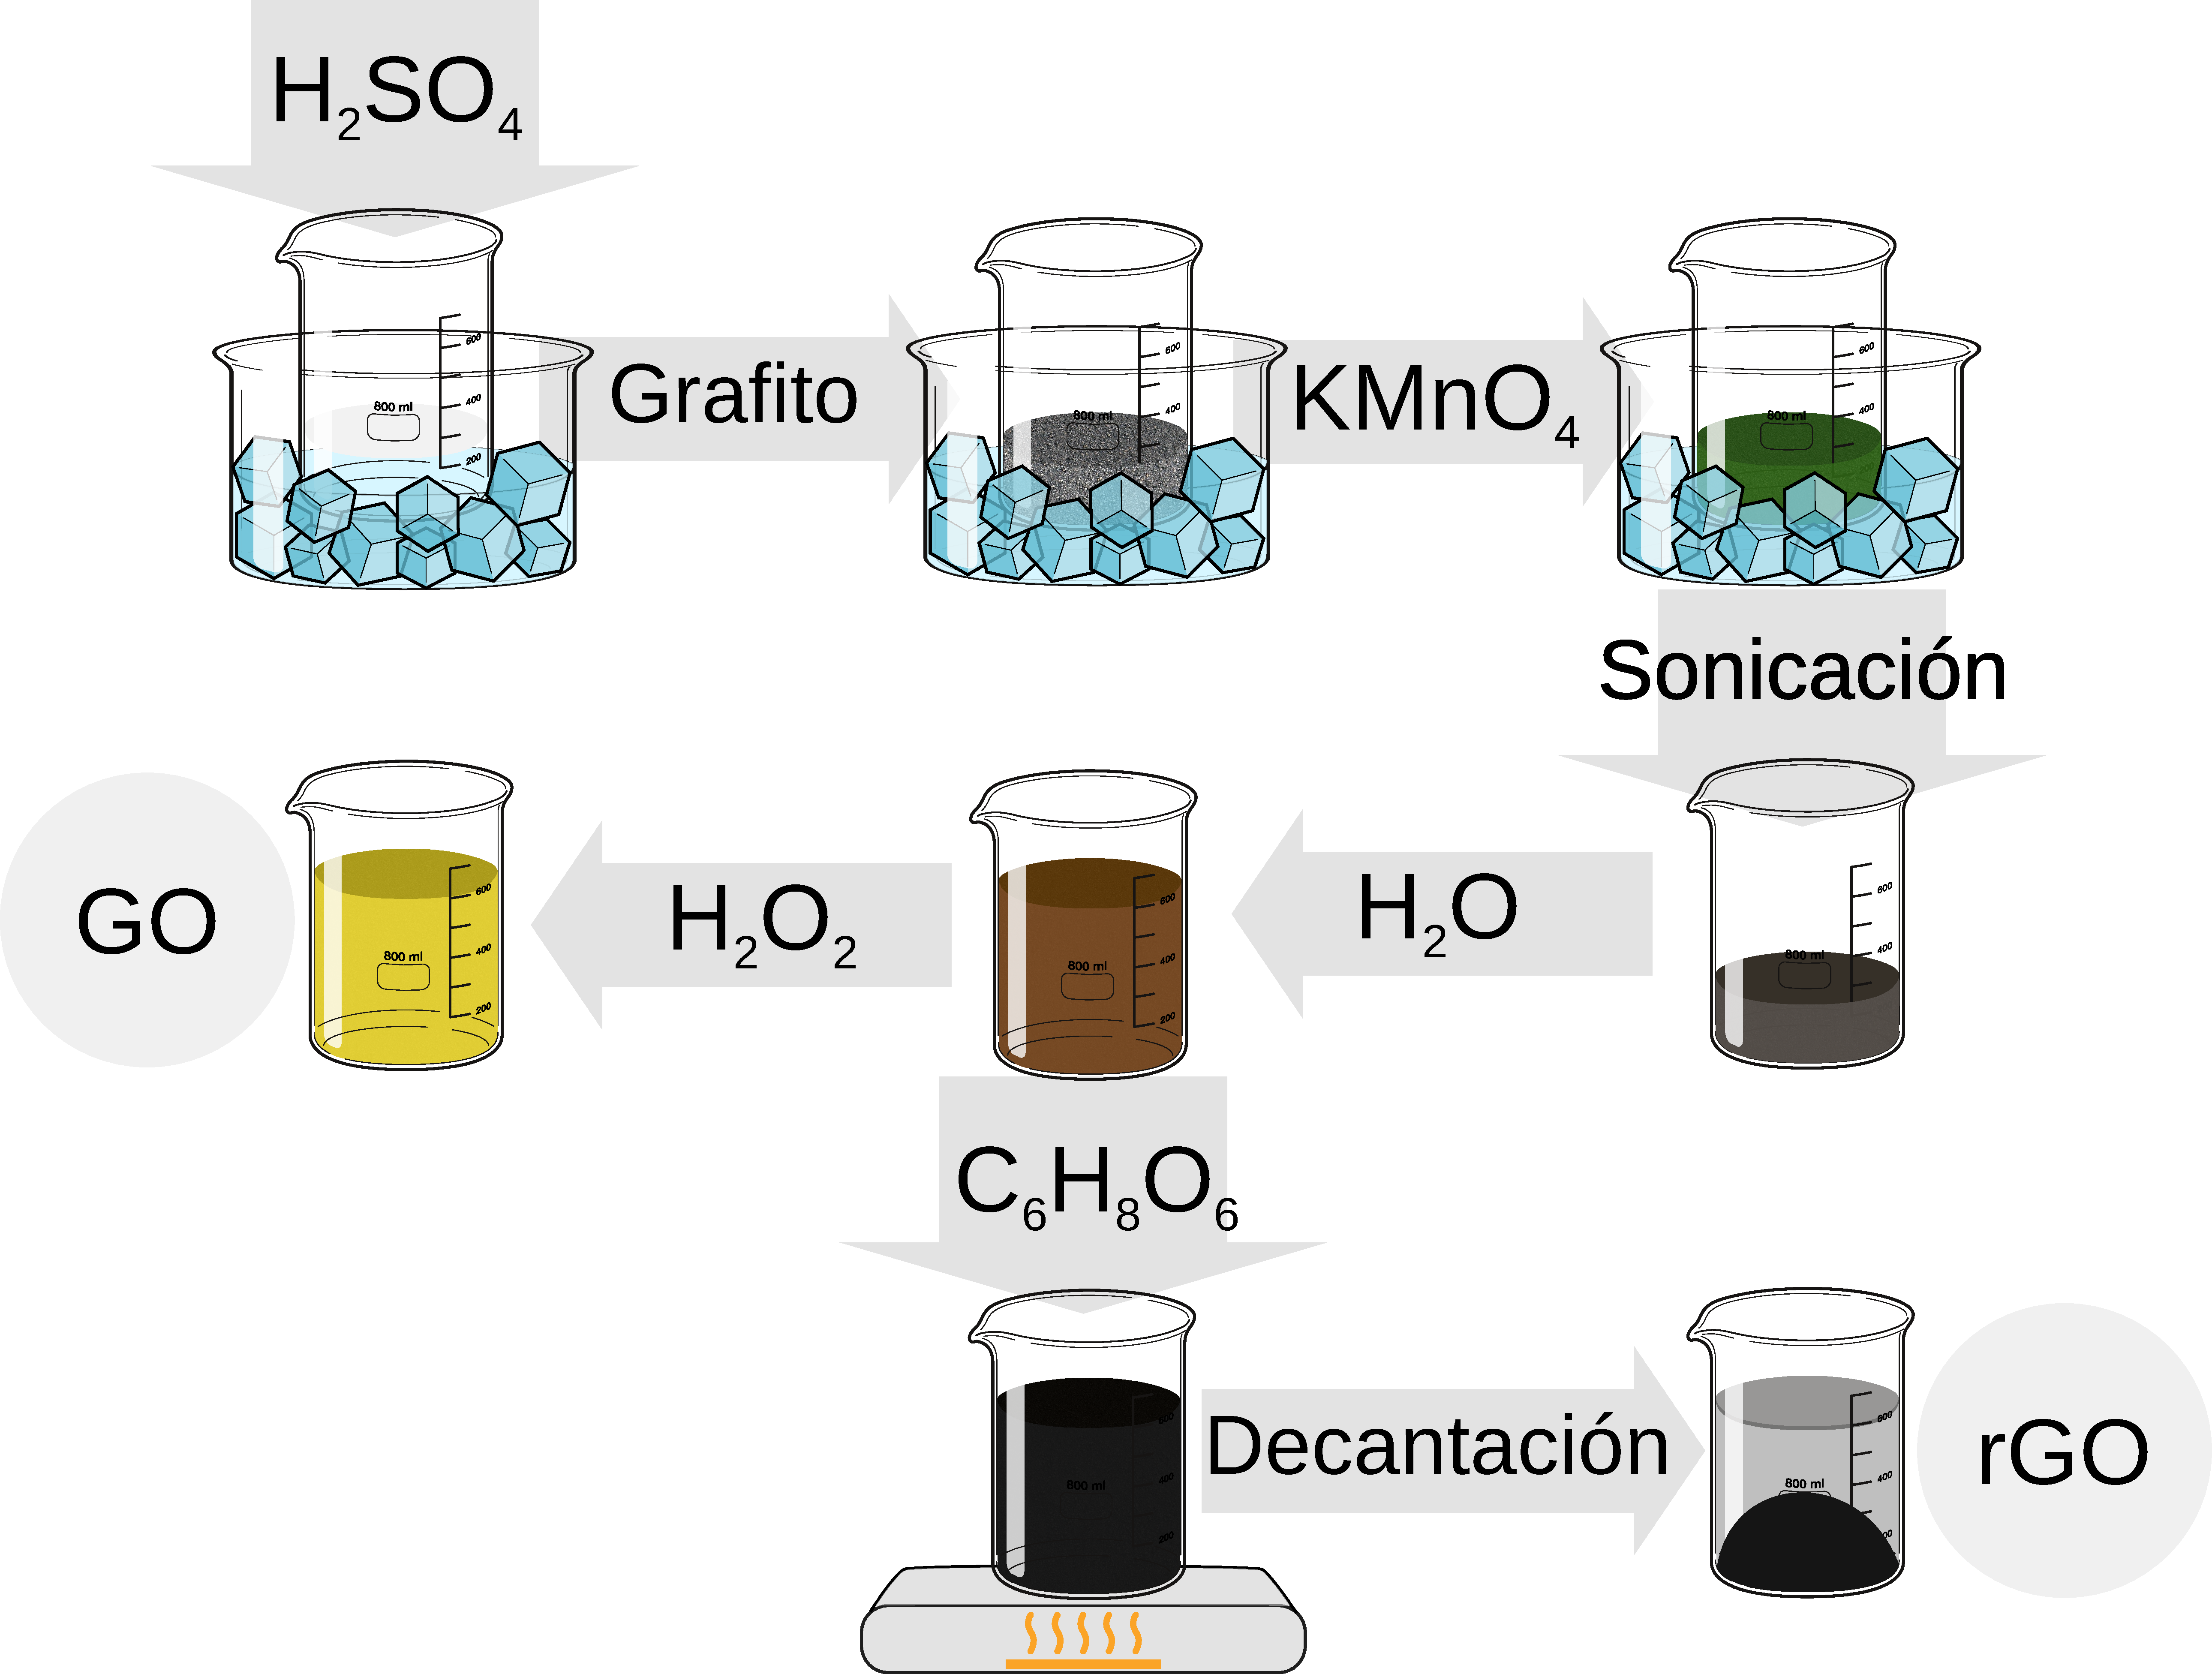
\includegraphics[width=\textwidth]{experimental_method.pdf}};
					\end{scope}}
				\only<8->{\begin{scope}
					\clip[] ( 3.5, -3.5) circle(\clipradius) ;
					\node at (0, -1) {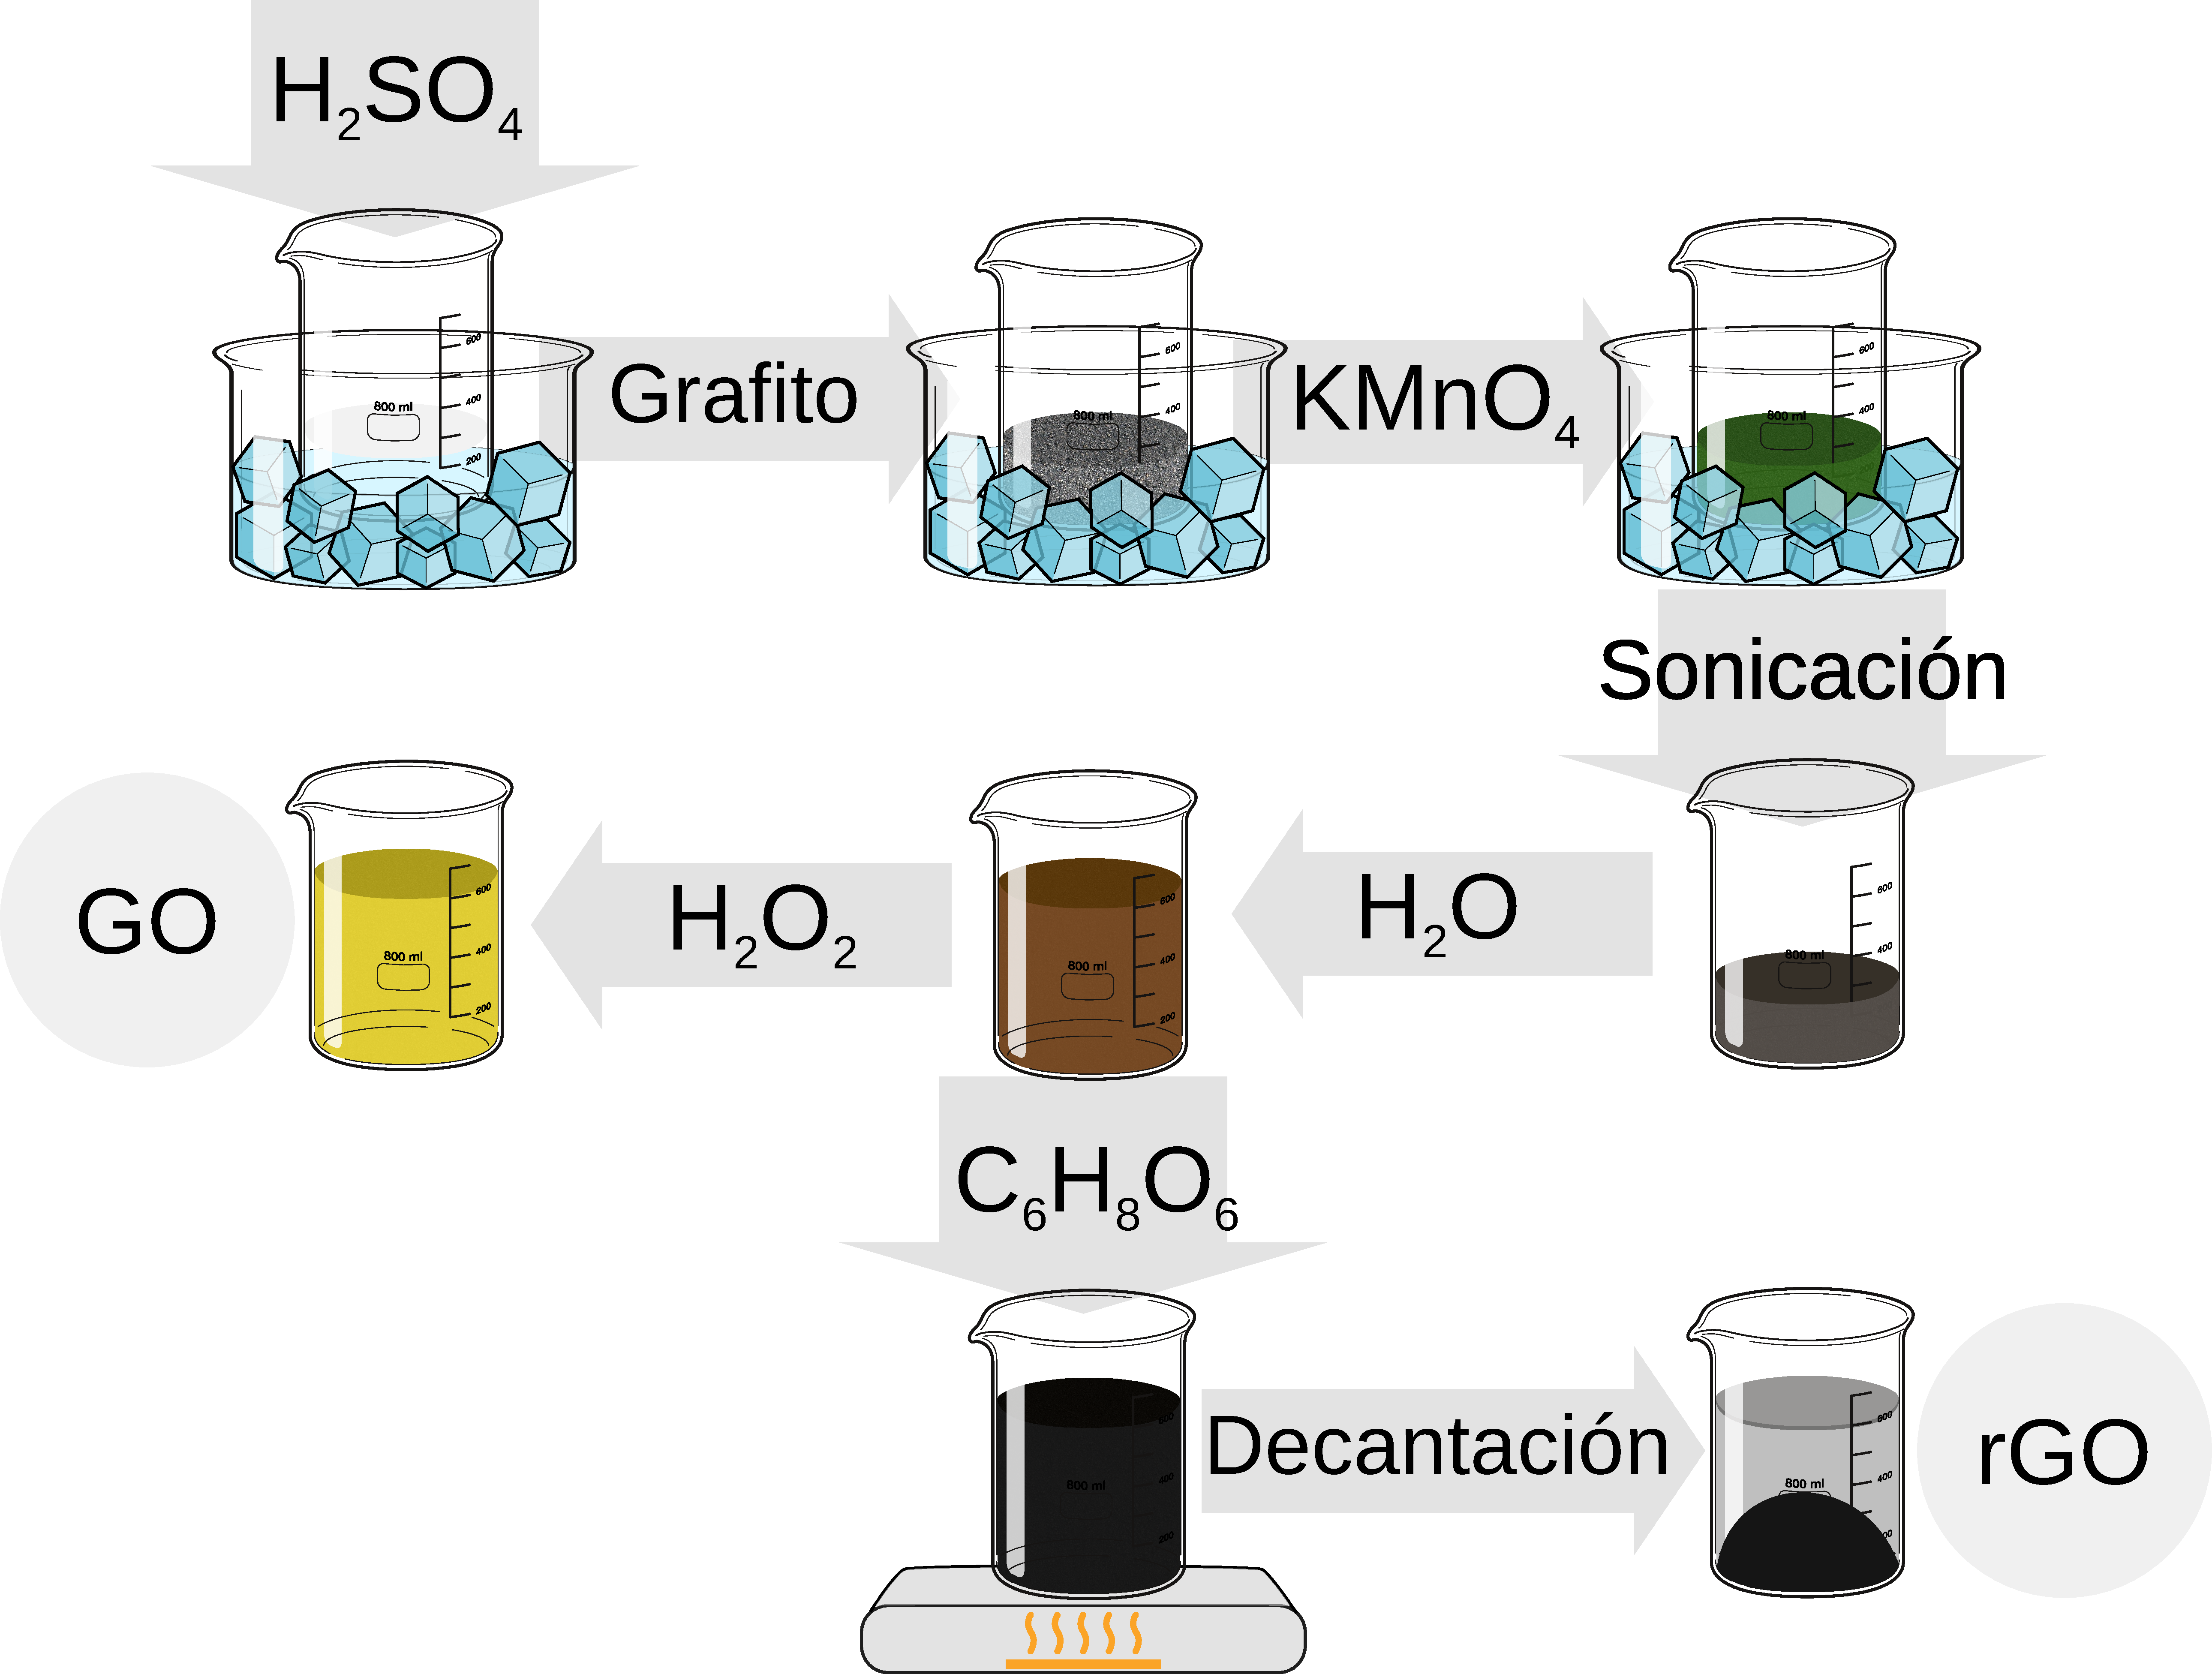
\includegraphics[width=\textwidth]{experimental_method.pdf}};
					\end{scope}}
			\end{tikzpicture}
		\end{figure}
	\end{frame}

	\begin{frame}{Resultados de la síntesis}
		\begin{figure}[h]
			\centering
			\fbox{
				\begin{subfigure}{0.4\textwidth}
					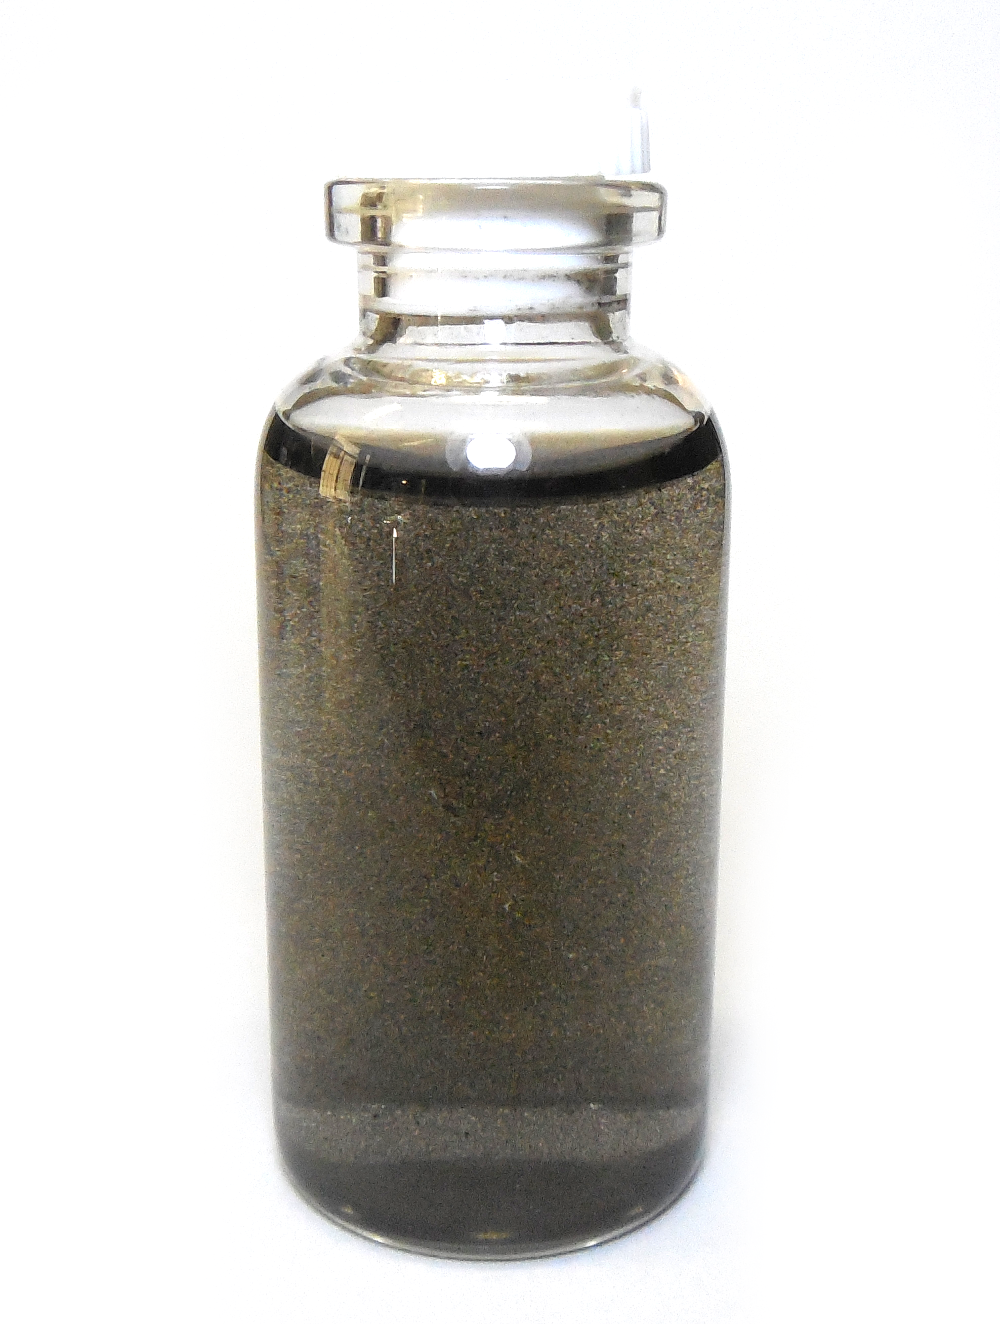
\includegraphics[width=\textwidth]{RGO_pic.png}
					\caption{rGO}
					\label{fig:RGO}
				\end{subfigure}
				\begin{subfigure}{0.42\textwidth}
					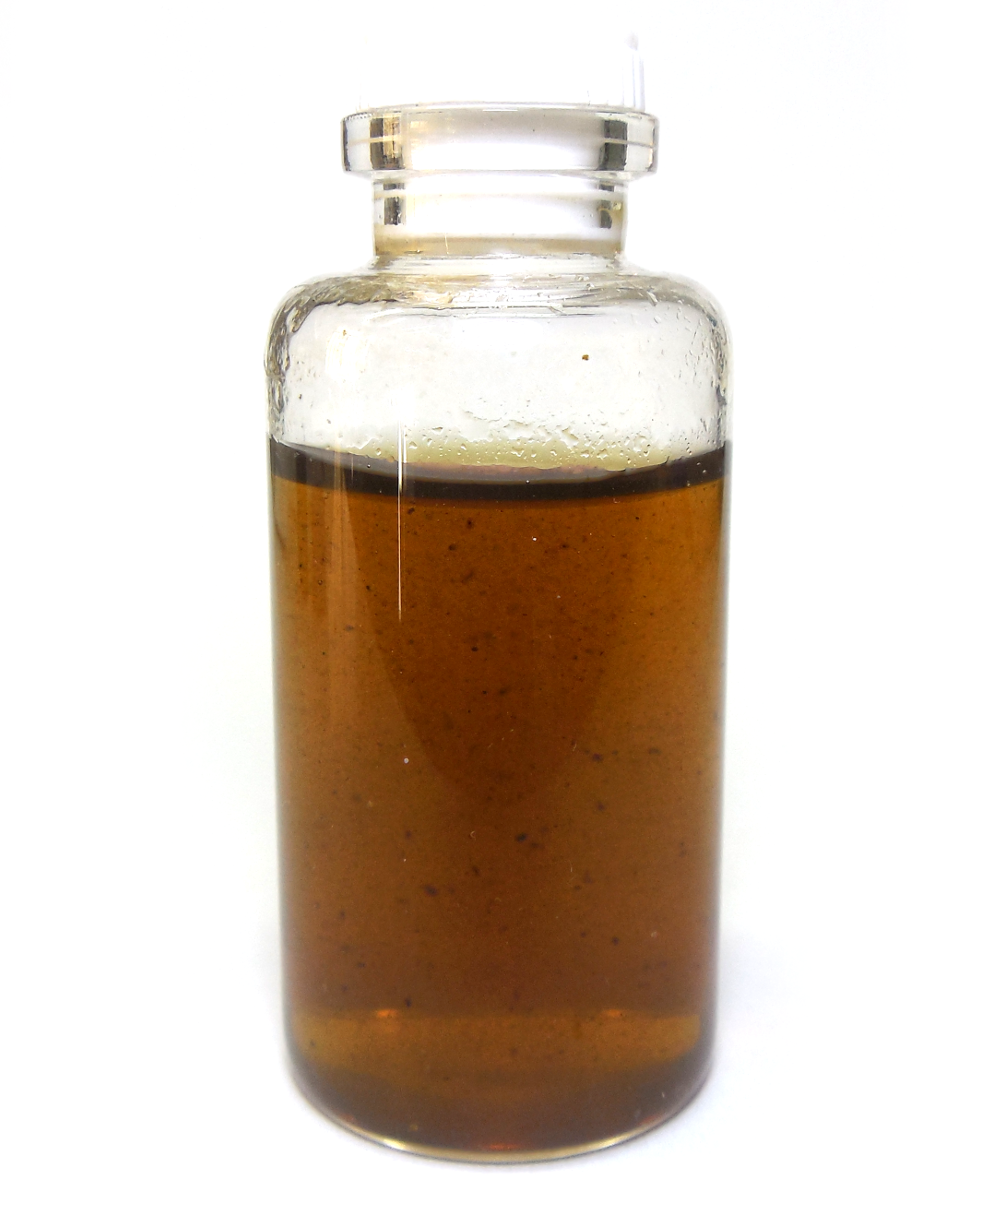
\includegraphics[width=\textwidth]{GO_pic.png}
					\caption{GO}
					\label{fig:GO}
				\end{subfigure}
			}
			\caption[Dispersiones de rGO y GO en agua]{Dispersiones de rGO y GO en agua.}
			\label{fig:RGOyGO}
		\end{figure}
	\end{frame}
	
	\begin{frame}{XRD}
		\begin{figure}[h]
			\centering
			\begin{tikzpicture}[]
			\begin{axis}[
			cycle list name=colorbrewer-RYB,
			no markers,
			width = 0.8\textwidth,
			yticklabels={,,},
			ylabel={Intensidad},
			y unit=u.a.,
			xlabel={2$\mathrm{\theta}$},
			x unit=grados,
			legend entries={Grafito, Óxido de grafeno, Óxido de grafeno reducido},
			legend style={font=\fontsize{4}{5}\selectfont},
			]
			\addplot table [x expr = \thisrow{2t}, y expr=\thisrow{C}] {./Data/XRD/xrd.txt};
			\addplot table [x expr = \thisrow{2t}, y expr=\thisrow{GO}+1] {./Data/XRD/xrd.txt};
			\pgfplotsset{cycle list shift=1}
			\addplot table [x expr = \thisrow{2t}, y expr=\thisrow{RGO}+2] {./Data/XRD/xrd.txt};
			%	\addplot table [x expr = \thisrow{2t}, y expr=\thisrow{RGOLYO}+3] {./Data/XRD/xrd.txt};
			\node[black, rotate=90] at (24, 0.3){\Tiny{(002)}};
			%	\node[black, rotate=90] at (7, 1.5){\small{10,2\degree}};
			%	\node[black, rotate=90] at (26, 3){\small{22,6\degree}};
			\end{axis}
			\end{tikzpicture}
			\caption[Espectro de difracción de rayos x de grafito, GO y rGO]{Espectro de difracción de rayos x.}
			\label{fig:xrd}
		\end{figure}
	\end{frame}

	\section{Supercondensadores}
	\begin{frame}{Construcción de supercondensadores}
		\begin{figure}[h!]
			\centering
			\fbox{
				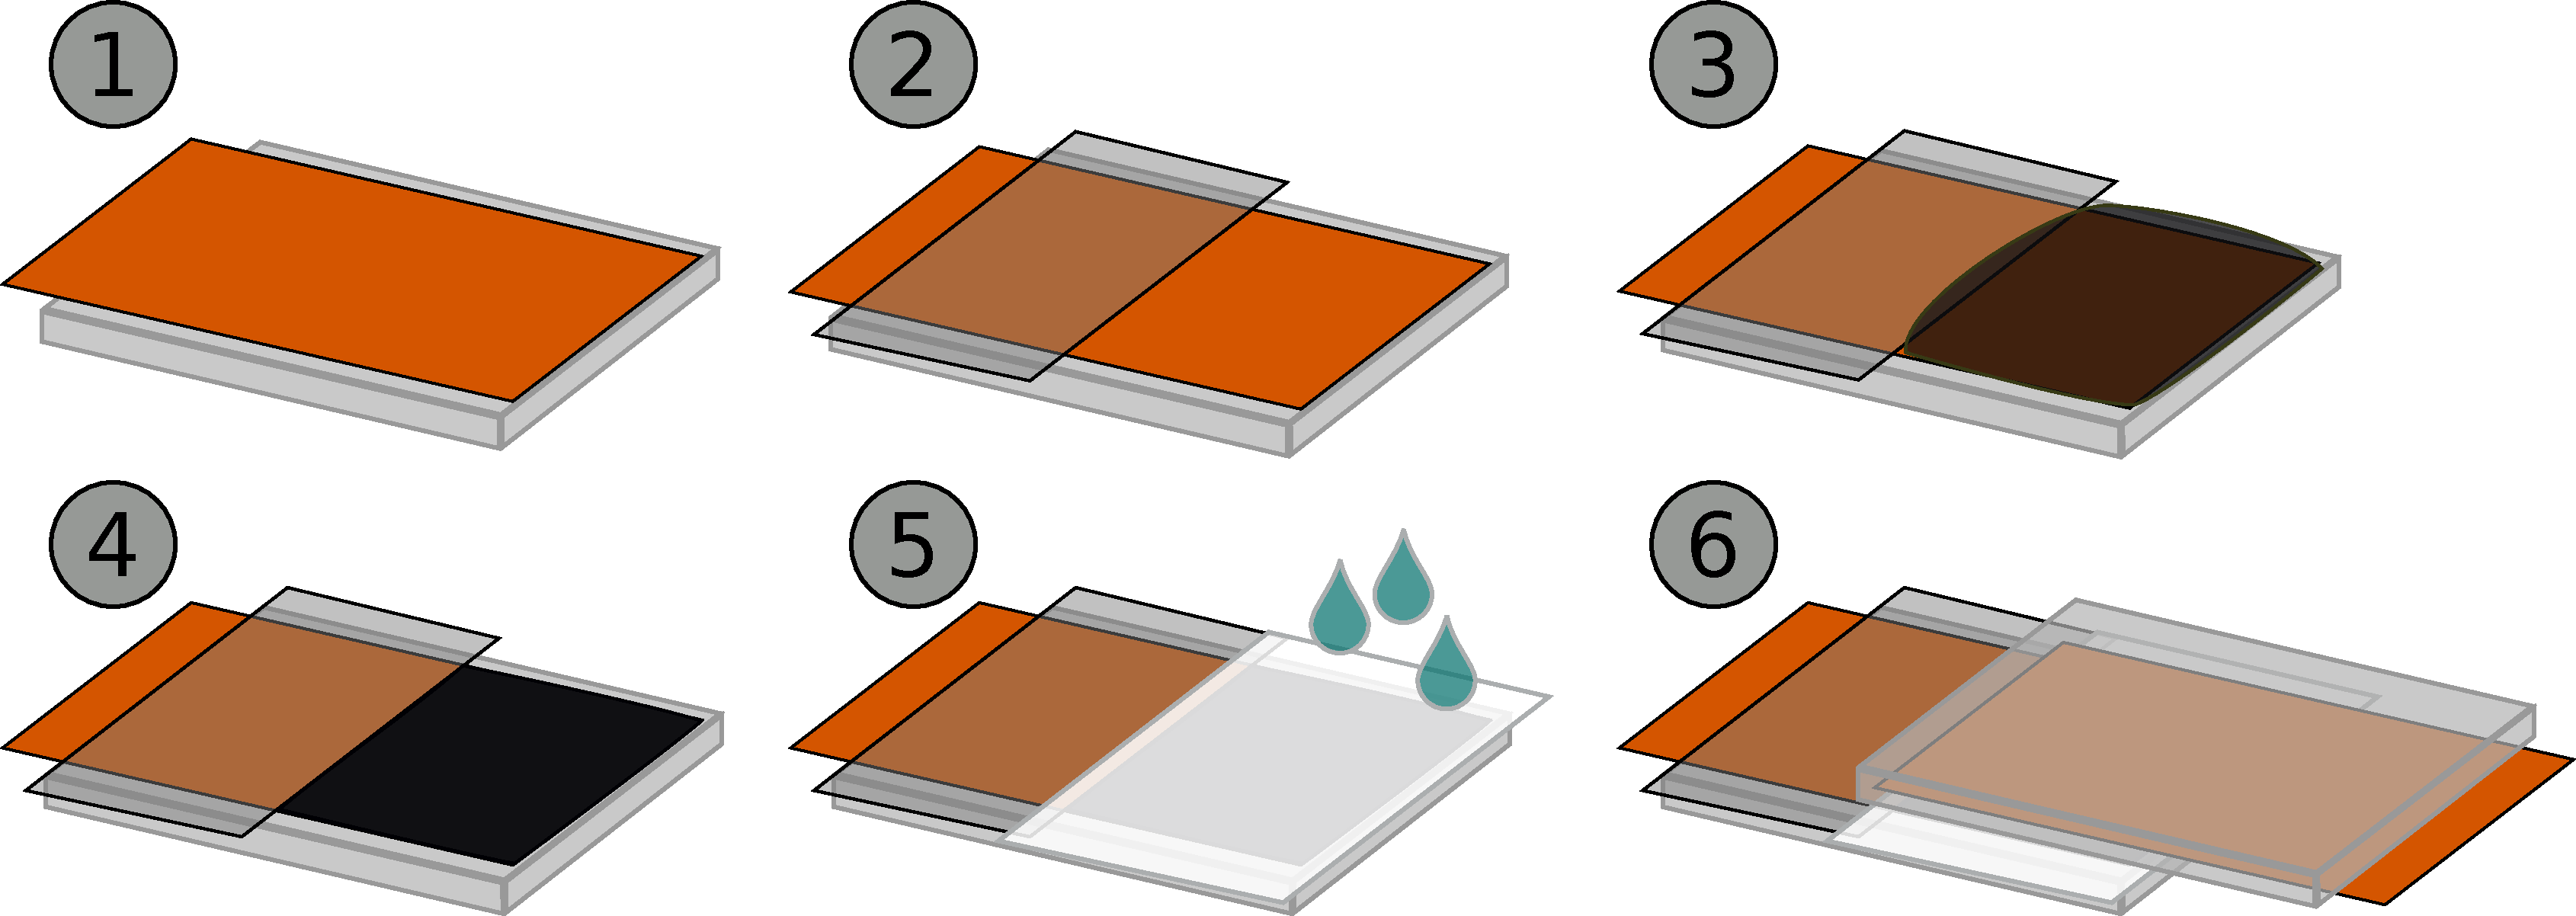
\includegraphics[width = 0.9\textwidth]{SC_process.pdf}
			}
			\caption[Principio de contrucción de un supercondensador]{Secuencia para la construcción de un supercondensador básico.}
			\label{fig:SC_process}
		\end{figure}
	\end{frame}

	\begin{frame}{Celda de pruebas}
		\begin{figure}[h!]
			\centering
			\fbox{
				\begin{subfigure}[b]{0.5\textwidth}
					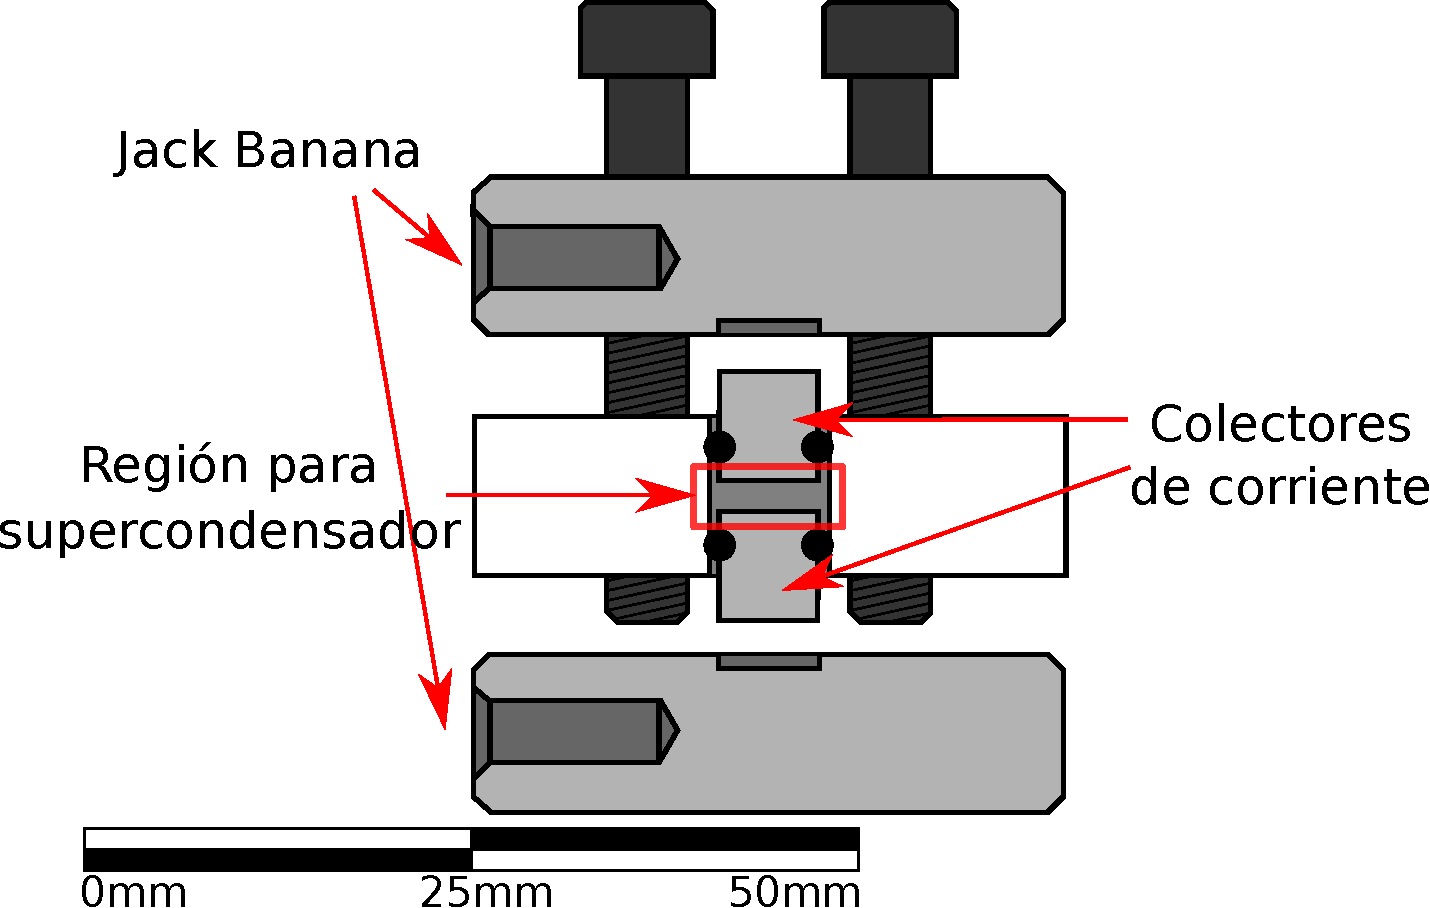
\includegraphics[width=\textwidth]{cell_scheme.pdf}
					\caption{}
					\label{fig:cell_scheme}
				\end{subfigure}\hspace{1cm}
				\begin{subfigure}[b]{0.25\textwidth}
					\includegraphics[width=\textwidth]{cell_image.pdf}
					\caption{}
					\label{fig:cell_image}
				\end{subfigure}
			}
			\caption[Celda de pruebas de supercondensador]{\subref{fig:cell_scheme} vista en corte longitudinal de la celda de pruebas mostrando los componentes más importantes. \subref{fig:cell_image} fotografía de la celda armada y conectada al potenciostato.}
			\label{fig:celda_de_pruebas_SC}
		\end{figure}
	\end{frame}
	
	\newcommand{\electrodesWidth}{0.22\textwidth}
	\begin{frame}{Construcción de electrodos}
		\begin{figure}
			\centering
			\begin{adjustbox}{minipage=0.7\linewidth,frame}
				\centering
				\begin{subfigure}[b]{\electrodesWidth}
					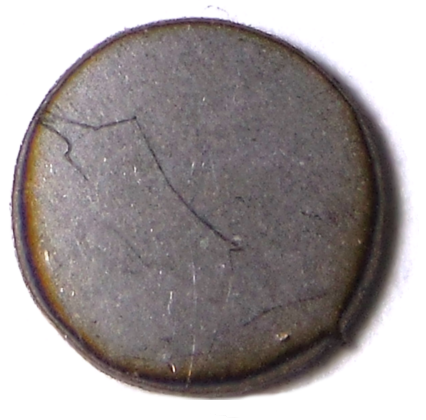
\includegraphics[width=\textwidth]{electrode_steel.png}
					\caption{\mSustratoAcero}
					\label{fig:substrate_steel}
				\end{subfigure}
				\begin{subfigure}[b]{\electrodesWidth}
					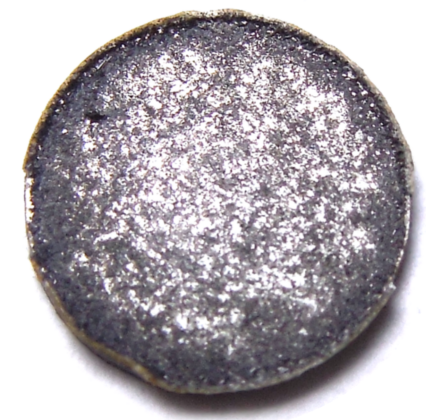
\includegraphics[width=\textwidth]{electrode_polvo_ac.png}
					\caption{\mPolvoAcero}
					\label{fig:electrode_powder_ac}
				\end{subfigure}
				\begin{subfigure}[b]{\electrodesWidth}
					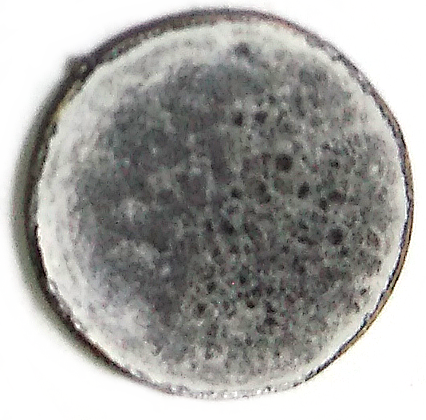
\includegraphics[width=\textwidth]{electrode_polvo_pmma_ac.png}
					\caption{\mPolvoAceroPMMA}
					\label{fig:electrode_powder_pmma_ac}
				\end{subfigure}
				\begin{subfigure}[b]{\electrodesWidth}
					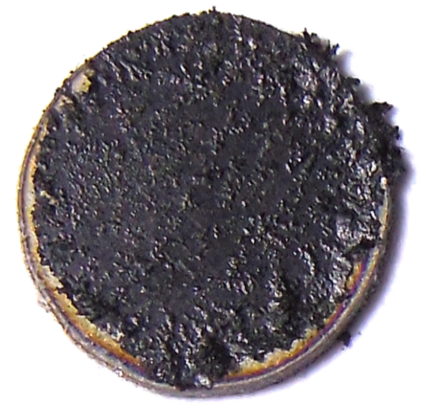
\includegraphics[width=\textwidth]{electrode_paper.png}
					\caption{\mPapelAcero}
					\label{fig:electrode_paper}
				\end{subfigure}\linebreak
				\begin{subfigure}[b]{\electrodesWidth}
					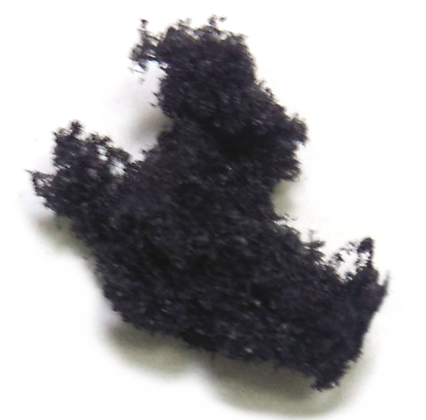
\includegraphics[width=\textwidth]{electrode_lio.png}
					\caption{\mLiofilizadoAcero}
					\label{fig:electrode_lio}
				\end{subfigure}
				\begin{subfigure}[b]{\electrodesWidth}
					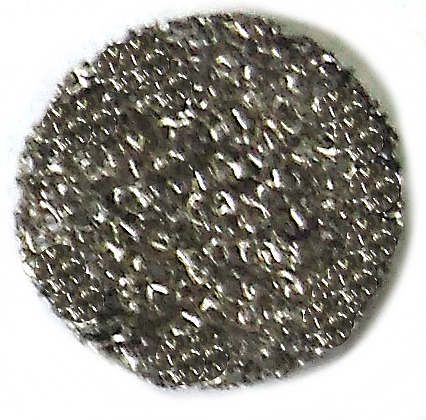
\includegraphics[width=\textwidth]{electrode_ni.png}
					\caption{\mSustratoNiquel}
					\label{fig:substrate_nickel}
				\end{subfigure}
				\begin{subfigure}[b]{\electrodesWidth}
					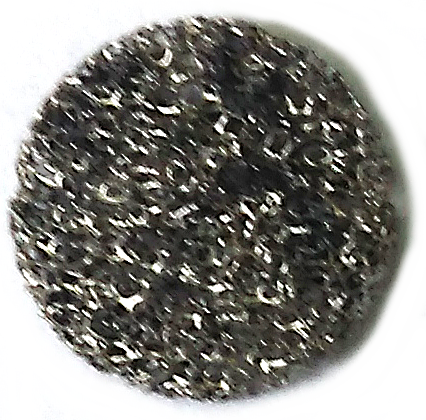
\includegraphics[width=\textwidth]{electrode_polvo_ni.png}
					\caption{\mPolvoNiquel}
					\label{fig:electrode_powder_ni}
				\end{subfigure}
				\begin{subfigure}[b]{\electrodesWidth}
					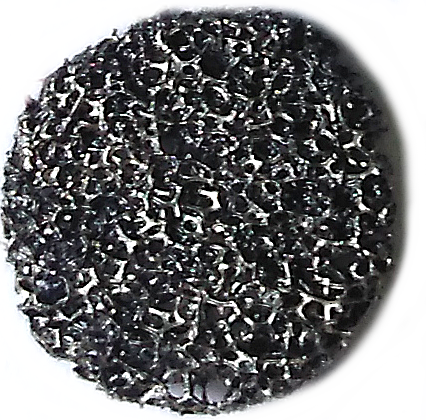
\includegraphics[width=\textwidth]{electrode_polvo_pmma_ni.png}
					\caption{\mPolvoNiquelPMMA}
					\label{fig:electrode_powder_pmma_ni}
				\end{subfigure}
			\end{adjustbox}
			\caption[Electrodos utilizados en la celda de pruebas de supercondensador]{Electrodos utilizados en la celda de pruebas de supercondensador.}
			\label{fig:electrodes}
		\end{figure}
	\end{frame}
	
	\begin{frame}{Caracterización electroquímica}
		\begin{table}[h!]
			\centering
			
			\begin{tabular}{ l r }
				Voltametría cíclica &  \\
				\hline
				Voltaje inicial [V] & 0 \\
				Límite inferior [V] & -0,8 \\
				Límite superior [V] & 0,8  \\
				Número de ciclos & 3 \\
				Velocidad de barrido [mV/s] & 25, 50, 100, 200, 400 \\
				& \\
				Carga y descarga cíclica & \\
				\hline
				Densidad de corriente [A/g] & 0,1 ó 	1 \\
				Número de ciclos & 1000 \\
				Límite inferior [V] & 0 \\
				Límite superior [V] & 1 \\
				& \\
				Espectroscopía de impedancia electroqúimica & \\
				\hline
				Frecuencia inicial	&	1 MHz \\
				Frecuencia final	&	0.1 Hz \\
				Corriente de exitación & 1 mA rms \\ 
			\end{tabular}
			\label{tab:elec_config}
			\caption[Parámetros de cada medición electroquímica]{Parámetros de cada medición electroquímica.}
		\end{table}
	\end{frame}

	\begin{frame}{Resultados}
		\begin{figure}[h!]
			\centering
			\begin{subfigure}[t!]{0.4\textwidth}
				\begin{tikzpicture}[scale=\plotscale,trim axis right,trim axis left]
				\begin{axis}
				[
				CVStyle,
				legend entries={\mPapelAcero, \mLiofilizadoAcero}
				]
				\addplot table [x=Voltaje, y expr=\thisrow{Corriente}/0.0006 ] {./Data/CV_CRGO300517_11/raw/sample3.txt};
				\addplot table [x=Voltaje, y expr=\thisrow{Corriente}/0.0006 ] {./Data/CV_CRGO300517_13/raw/sample3.txt};
				\end{axis}
				\end{tikzpicture}
%				\subcaption{Antes de 1000 ciclos de carga y descarga.}
			\end{subfigure}
			\begin{subfigure}[t!]{0.4\textwidth}
				\begin{tikzpicture}[scale=\plotscale,trim axis right,trim axis left]
				\begin{axis}[
				CVStyle,
				legend entries={\mPolvoAcero, \mPolvoAceroPMMA, \mPolvoNiquel, \mPolvoNiquelPMMA},
				cycle list shift=2
				]
				\addplot table [x=Voltaje, y expr=\thisrow{Corriente}/0.0004 ] {./Data/CV_CRGO300517_9/raw/sample3.txt};
				\addplot table [x=Voltaje, y expr=\thisrow{Corriente}/0.0028 ] {./Data/CV_CRGO300517_3/raw/sample3.txt};
				\addplot table [x=Voltaje, y expr=\thisrow{Corriente}/0.0009 ] {./Data/CV_CRGO300517_5/raw/sample3.txt};
				\addplot table [x=Voltaje, y expr=\thisrow{Corriente}/0.0008 ] {./Data/CV_CRGO300517_7/raw/sample3.txt};	
				\end{axis}
				\end{tikzpicture}
%				\subcaption{Antes de 1000 ciclos de carga y descarga.}
			\end{subfigure}
			\begin{subfigure}[t!]{0.4\textwidth}
				\begin{tikzpicture}[scale=\plotscale,trim axis right,trim axis left]
				\begin{axis}[
				CVStyle,
				legend entries={\mPapelAcero, \mLiofilizadoAcero}
				]
				\addplot table [x=Voltaje, y expr=\thisrow{Corriente}/0.0006 ] {./Data/CV_CRGO300517_12/raw/sample3.txt};
				\addplot table [x=Voltaje, y expr=\thisrow{Corriente}/0.0006 ] {./Data/CV_CRGO300517_14/raw/sample3.txt};	
				\end{axis}
				\end{tikzpicture}
%				\subcaption{Después de 1000 ciclos de carga y descarga.}
			\end{subfigure}
			\begin{subfigure}[t!]{0.4\textwidth}
				\begin{tikzpicture}[scale=\plotscale,trim axis right,trim axis left]
				\begin{axis}[
				CVStyle,
				legend entries={\mPolvoAcero, \mPolvoAceroPMMA, \mPolvoNiquel, \mPolvoNiquelPMMA},
				cycle list shift=2
				] 
				\addplot table [x=Voltaje, y expr=\thisrow{Corriente}/0.0004 ] {./Data/CV_CRGO300517_10/raw/sample3.txt};
				\addplot table [x=Voltaje, y expr=\thisrow{Corriente}/0.0028 ] {./Data/CV_CRGO300517_4/raw/sample3.txt};
				\addplot table [x=Voltaje, y expr=\thisrow{Corriente}/0.0009 ] {./Data/CV_CRGO300517_6/raw/sample3.txt};
				\addplot table [x=Voltaje, y expr=\thisrow{Corriente}/0.0008 ] {./Data/CV_CRGO300517_7/raw/sample3.txt};
				\end{axis}
				\end{tikzpicture}
%				\subcaption{Después de 1000 ciclos de carga y descarga.}
			\end{subfigure}
			\caption[Resumen voltametría cíclica a 100 mV/s antes y después de 1000 ciclos de carga y descarga]{Resumen voltametría cíclica a 100 mV/s antes y después de 1000 ciclos de carga y descarga. Las muestras son separadas en dos gráficos para mejorar su visualización.}
			\label{fig:resumen_cv}
		\end{figure}
	\end{frame}

	\begin{frame}{Resumen Capacitancia}
		\begin{table}[h!]
			\centering
			\caption{Resumen de capacitancia y capacitancia específica a 100 mV/s.}
			\begin{tabular}{ l l c c c }
				\multirow{2}{*}{Muestra}& \multirow{2}{*}{Masa [mg]}& \multirow{2}{*}{Capacitancia [mF]}	& Capacitancia & \multirow{2}{*}{Error}\\
				&         			      & 										& específica [F/g]     &			\\
				\hline
				\mSustratoAcero		&  -            &			0.1			&	-				&	-		\\
				\mPolvoAcero		& 0,4 $\pm$ 0,2 &			1.2			&	3.0	$\pm$ 1.5	&	50\%	\\
				\mPolvoAceroPMMA	& 2,8 $\pm$ 0,2 &			0.78		&	0.28 $\pm$ 0.02	&	7\%		\\
				\rowcolor{RYB3}
				\mPapelAcero		& 0,6 $\pm$ 0,1 &			16.8		&	28.0 $\pm$ 4.7	&	17\%	\\
				\rowcolor{RYB3}
				\mLiofilizadoAcero	& 0,6 $\pm$ 0,1 &			19.9		&	33.2 $\pm$ 5.5	&	17\%	\\
				\mSustratoNiquel	&    -          &			0.1			&	- 				&	-		\\
				\mPolvoNiquel		& 0,9 $\pm$ 0,2 &			0.3			&	0.35 $\pm$ 0.07	&	20\%	\\
				\mPolvoNiquelPMMA	& 0,8 $\pm$ 0,2 &			1.2			&	1.5	$\pm$ 0.4	&	27\%	\\
			\end{tabular}                                                          
			\label{tab:resumen_capacitancia}
		\end{table}
	\end{frame}

	\begin{frame}{EIS}
		\begin{figure}[h!]
			\centering
			\begin{subfigure}[t!]{0.4\textwidth}
				\begin{tikzpicture}[scale=\plotscale,trim axis right,trim axis left]
				\begin{axis}[
				EISStyle,
				every axis legend/.append style={
					font=\tiny,
					at={(0.02,0.98)},
					anchor=north west,
				},
				legend entries = {\mPapelAcero, \mLiofilizadoAcero}
				]
				\pgfplotstableread{./Data/CV_CRGO300517_11/raw/eisgalv.txt}{\eistable};
				\pgfplotstablegetrowsof{\eistable}
				\pgfmathsetmacro{\N}{\pgfplotsretval}
				\addplot table [only marks, x=Zreal, y expr=\thisrow{Zimag}*-1] {\eistable}
				node[pos=(1-1)/(\N-1), pin=right:{1 MHz}]{}
				node[pos=(\N-1)/(\N-1), pin=left:{0,1 Hz}]{};
				\pgfplotstableread{./Data/CV_CRGO300517_13/raw/eisgalv.txt}{\eistable};
				\pgfplotstablegetrowsof{\eistable}
				\addplot table [only marks, x=Zreal, y expr=\thisrow{Zimag}*-1] {\eistable}
				node[pos=(1-1)/(\N-1), pin=right:{1 MHz}]{}
				node[pos=(40-1)/(\N-1), ]{}
				node[pos=(\N-1)/(\N-1), pin=left:{0,1 Hz}]{};
				\end{axis}
				\end{tikzpicture}
			\end{subfigure}\hfill
			\begin{subfigure}[t!]{0.4\textwidth}
				\begin{tikzpicture}[scale=\plotscale,trim axis right,trim axis left]
				\begin{axis}[
				EISStyle,
				every axis legend/.append style={
					font=\tiny,
					at={(0.98,0.02)},
					anchor=south east,
				},
				legend entries = {\mPolvoAcero, \mPolvoAceroPMMA, \mPolvoNiquel, \mPolvoNiquelPMMA},
				cycle list shift=2
				]
				\pgfplotstableread{./Data/CV_CRGO300517_9/raw/eisgalv.txt}{\eistable};
				\pgfplotstablegetrowsof{\eistable}
				\pgfmathsetmacro{\N}{\pgfplotsretval}
				\addplot table [only marks, x=Zreal, y expr=\thisrow{Zimag}*-1] {\eistable}
				node[pos=(1-1)/(\N-1), pin=right:{1 MHz}]{}
				node[pos=(\N-1)/(\N-1), pin=left:{0,1 Hz}]{};
				\pgfplotstableread{./Data/CV_CRGO300517_3/raw/eisgalv.txt}{\eistable};
				\pgfplotstablegetrowsof{\eistable}
				\addplot table [only marks, x=Zreal, y expr=\thisrow{Zimag}*-1] {\eistable}
				node[pos=(1-1)/(\N-1), pin=right:{1 MHz}]{}
				node[pos=(\N-1)/(\N-1), pin=left:{0,1 Hz}]{};
				\pgfplotstableread{./Data/CV_CRGO300517_5/raw/eisgalv.txt}{\eistable};
				\pgfplotstablegetrowsof{\eistable}
				\addplot table [only marks, x=Zreal, y expr=\thisrow{Zimag}*-1] {\eistable}
				node[pos=(1-1)/(\N-1), pin=right:{1 MHz}]{}
				node[pos=(\N-1)/(\N-1), pin=left:{0,1 Hz}]{};
				\pgfplotstableread{./Data/CV_CRGO300517_7/raw/eisgalv.txt}{\eistable};
				\pgfplotstablegetrowsof{\eistable}
				\addplot table [only marks, x=Zreal, y expr=\thisrow{Zimag}*-1] {\eistable}
				node[pos=(1-1)/(\N-1), pin=right:{1 MHz}]{}
				node[pos=(\N-1)/(\N-1), pin=left:{0,1 Hz}]{};
				\end{axis}
				\end{tikzpicture}
			\end{subfigure}
			\caption[Resumen del espectro de impedancia electroquímica]{Resumen del espectro de impedancia electroquímica. Las muestras son separadas en dos gráficos para mejorar su visualización.}
			\label{fig:resumen_eis}
		\end{figure}
	\end{frame}
	
	\begin{frame}{Carga y descarga}
		\begin{figure}[h!]
			\centering
			\begin{subfigure}{0.4\textwidth}
				\begin{tikzpicture}[scale=\plotscale,trim axis right,trim axis left]
				\begin{axis}[CCDStyle,
				every axis legend/.append style={
					font=\tiny,
					at={(0.98,0.98)},
					anchor=north east,
				},
				legend entries={\mPapelAcero, \mLiofilizadoAcero}]
				%		\addplot+[restrict x to domain=0:4.146667] table [ x expr=\thisrow{Time}-5.22166600000000, y expr=\thisrow{Voltage} ] {./Data/CV_CRGO300517_9/raw/chargedischarge.txt};
				%		\addplot+[restrict x to domain=0:5.748327] table [ x expr=\thisrow{Time}-12.7000030000000, y expr=\thisrow{Voltage} ] {./Data/CV_CRGO300517_3/raw/chargedischarge.txt};
				\addplot+[restrict x to domain=0:62.000063] table [ x expr=\thisrow{Time}-63.3333370000000, y expr=\thisrow{Voltage} ] {./Data/CV_CRGO300517_11/raw/chargedischarge.txt};
				\addplot+[restrict x to domain=0:113.320033] table [ x expr=\thisrow{Time}-138.664967000000, y expr=\thisrow{Voltage} ] {./Data/CV_CRGO300517_13/raw/chargedischarge.txt};
				%		\addplot+[restrict x to domain=0:5.743334] table [ x expr=\thisrow{Time}-5.48000000000000, y expr=\thisrow{Voltage} ] {./Data/CV_CRGO300517_5/raw/chargedischarge.txt};
				%		\addplot+[restrict x to domain=0:1.088334] table [ x expr=\thisrow{Time}-2.29000000000000, y expr=\thisrow{Voltage} ] {./Data/CV_CRGO300517_7/raw/chargedischarge.txt};
				\end{axis}
				\end{tikzpicture}
			\end{subfigure}\hfill
			\begin{subfigure}{0.4\textwidth}
				\begin{tikzpicture}[scale=\plotscale,trim axis right,trim axis left]
				\begin{axis}[CCDStyle,
				every axis legend/.append style={
					font=\tiny,
					at={(0.68,0.88)},
					anchor=north west,
				},
				legend entries={\mPolvoAcero, \mPolvoAceroPMMA, \mPolvoNiquel, \mPolvoNiquelPMMA},
				cycle list shift=2
				]
				\addplot+[restrict x to domain=0:4.146667] table [ x expr=\thisrow{Time}-5.22166600000000, y expr=\thisrow{Voltage} ] {./Data/CV_CRGO300517_9/raw/chargedischarge.txt};
				\addplot+[restrict x to domain=0:5.748327] table [ x expr=\thisrow{Time}-12.7000030000000, y expr=\thisrow{Voltage} ] {./Data/CV_CRGO300517_3/raw/chargedischarge.txt};
				%		\addplot+[restrict x to domain=0:62.000063] table [ x expr=\thisrow{Time}-63.3333370000000, y expr=\thisrow{Voltage} ] {./Data/CV_CRGO300517_11/raw/chargedischarge.txt};
				%		\addplot+[restrict x to domain=0:113.320033] table [ x expr=\thisrow{Time}-138.664967000000, y expr=\thisrow{Voltage} ] {./Data/CV_CRGO300517_13/raw/chargedischarge.txt};
				\addplot+[restrict x to domain=0:5.743334] table [ x expr=\thisrow{Time}-5.48000000000000, y expr=\thisrow{Voltage} ] {./Data/CV_CRGO300517_5/raw/chargedischarge.txt};
				\addplot+[restrict x to domain=0:1.088334] table [ x expr=\thisrow{Time}-2.29000000000000, y expr=\thisrow{Voltage} ] {./Data/CV_CRGO300517_7/raw/chargedischarge.txt};
				\end{axis}
				\end{tikzpicture}
			\end{subfigure}
			\caption[Resumen de carga y descarga cíclica]{Resumen de carga y descarga cíclica a 1 A/g, exceptuando las muestras de polvo más pmma en disco de acero y polvo en espuma de níquel donde la densidad de corriente es de 0,1 A/g. Las muestras son separadas en dos gráficos para mejorar su visualización.}
			\label{fig:resumen_ccd}
		\end{figure}
	\end{frame}

	\begin{frame}
		\begin{table}[h!]
			\centering
			\caption{Resistencia en serie equivalente calculada de los ciclos de carga y descarga.}
			\begin{tabular}{l c c c c}
				Muestra	&	$\mathrm{V_1}$ [mV]	&	$\mathrm{V_2}$ [mV]	&	Corriente [mA]	&	Resistencia [$\Omega$]	\\
				\hline
				\mPolvoAceroPMMA		&	1.000	&	596	&	-0,279	&	1.447	\\
				\mPolvoNiquel			&	1.000	&	854	&	-0,088	&	1.656	\\
				\mPolvoNiquelPMMA		&	999		&	402	&	-0,799	&	748		\\
				\mPolvoAcero			&	1.000	&	719	&	-0,398	&	705		\\
				\mPapelAcero			&	996		&	911	&	-0,599	&	141		\\
				\mLiofilizadoAcero		&	1.000	&	909	&	-0,599	&	150		\\
			\end{tabular}
			\label{tab:esr}
		\end{table}
	\end{frame}

	\begin{frame}
		\begin{figure}[h]
			\centering
			\begin{subfigure}[t]{0.4\textwidth}
				\begin{tikzpicture}[scale=\plotscale,trim axis right,trim axis left]
				\begin{semilogxaxis}[
				SCStyle,
				only marks,
				xtick = {25, 50, 100, 200, 400},
				xticklabels = {25, 50, 100, 200, 400},
				ylabel = {Capacidad específica [F/g]},
				ymin = 0,
				ymax = 50,
				every axis legend/.append style={
					font=\tiny,
					at={(0.98,0.98)},
					anchor=north east,
				},
				legend entries={\mPapelAcero, \mLiofilizadoAcero, \mPolvoAcero, \mPolvoAceroPMMA, \mPolvoNiquel, \mPolvoNiquelPMMA},
				]
				\addplot+ [error bars/.cd, y dir=both, y fixed relative=0.16666666666] table [y expr=\thisrow{Capacitancia}] {./Data/CV_CRGO300517_11/raw/capacitance.txt};
				\addplot+ [error bars/.cd, y dir=both, y fixed relative=0.16666666666] table [y expr=\thisrow{Capacitancia}] {./Data/CV_CRGO300517_13/raw/capacitance.txt};
				\addplot+ [error bars/.cd, y dir=both, y fixed relative=0.5] table [y expr=\thisrow{Capacitancia}] {./Data/CV_CRGO300517_9/raw/capacitance.txt};
				\addplot+ [error bars/.cd, y dir=both, y fixed relative=0.07142857142] table [y expr=\thisrow{Capacitancia}] {./Data/CV_CRGO300517_3/raw/capacitance.txt};
				\addplot+ [error bars/.cd, y dir=both, y fixed relative=0.22222222222] table [y expr=\thisrow{Capacitancia}] {./Data/CV_CRGO300517_5/raw/capacitance.txt};
				\addplot+ [error bars/.cd, y dir=both, y fixed relative=0.25] table [y expr=\thisrow{Capacitancia}] {./Data/CV_CRGO300517_7/raw/capacitance.txt};
				
				\end{semilogxaxis}
				\end{tikzpicture}
				\caption{Capacidad específica antes de 1000 ciclos de carga y descarga. }
			\end{subfigure}\hfill
			\begin{subfigure}[t]{0.4\textwidth}
				\begin{tikzpicture}[scale=\plotscale,trim axis right,trim axis left]
				\begin{semilogxaxis}[
				SCStyle,
				only marks,
				xtick = {25, 50, 100, 200, 400},
				xticklabels = {25, 50, 100, 200, 400},
				ylabel = {Capacidad específica [F/g]},
				ymin = 0,
				ymax = 50,
				every axis legend/.append style={
					font=\tiny,
					at={(0.98,0.98)},
					anchor=north west,
				},
				legend entries={\mPapelAcero, \mLiofilizadoAcero, \mPolvoAcero, \mPolvoAceroPMMA, \mPolvoNiquel, \mPolvoNiquelPMMA},
				]
				\addplot+ [error bars/.cd, y dir=both, y fixed relative=0.16666666666] table [y expr=\thisrow{Capacitancia}] {./Data/CV_CRGO300517_12/raw/capacitance.txt};
				\addplot+ [error bars/.cd, y dir=both, y fixed relative=0.16666666666] table [y expr=\thisrow{Capacitancia}] {./Data/CV_CRGO300517_14/raw/capacitance.txt};
				\addplot+ [error bars/.cd, y dir=both, y fixed relative=0.50000000000] table [y expr=\thisrow{Capacitancia}] {./Data/CV_CRGO300517_10/raw/capacitance.txt};
				\addplot+ [error bars/.cd, y dir=both, y fixed relative=0.07142857142] table [y expr=\thisrow{Capacitancia}] {./Data/CV_CRGO300517_4/raw/capacitance.txt};
				\addplot+ [error bars/.cd, y dir=both, y fixed relative=0.22222222222] table [y expr=\thisrow{Capacitancia}] {./Data/CV_CRGO300517_6/raw/capacitance.txt};
				\addplot+ [error bars/.cd, y dir=both, y fixed relative=0.25000000000] table [y expr=\thisrow{Capacitancia}] {./Data/CV_CRGO300517_8/raw/capacitance.txt};
				
				\end{semilogxaxis}
				\end{tikzpicture}
				\caption{Capacidad específica después de 1000 ciclos de carga y descarga. }
			\end{subfigure}
			\caption[Resumen de la capacidad específica]{Resumen de la capacidad específica.}
			\label{fig:resumen_cs}
		\end{figure}x
	\end{frame}

	\section{Bibliografía}
	\begin{frame}{Bibliografía}
		\bibliography{Nanosintesis}
		\bibliographystyle{apalike}
		
	\end{frame}

	\maketitle

\end{document}